\documentclass[11pt,a4paper]{article}
\usepackage[T1]{fontenc}
\usepackage[utf8]{inputenc}
\usepackage{mathpazo}
\usepackage[a4paper,left=2.47cm,right=2.47cm,top=2.5cm,bottom=2.6cm]{geometry}
\usepackage{amsmath,amssymb}
\usepackage{graphicx}
\usepackage{booktabs}
\usepackage{array}
\usepackage{tabularx}
\usepackage{multirow}
\usepackage{adjustbox}
\usepackage{enumitem}
\usepackage[labelsep=period,font=small,labelfont=bf]{caption}
\usepackage[authoryear,round]{natbib}
\usepackage{xcolor}
\usepackage[colorlinks=true,linkcolor=black,citecolor=black,urlcolor=black]{hyperref}
\usepackage{xurl}
\usepackage{microtype}
\setlength{\emergencystretch}{2.5em}
\setlist{itemsep=2pt,topsep=4pt}
\setlength{\parskip}{0pt}
\renewcommand{\arraystretch}{1.05}
\newcommand{\figw}{\textwidth}
\newcommand{\sym}[1]{\ensuremath{#1}}
\newcommand{\para}[1]{\par\medskip\noindent\textbf{#1}\quad}
\hypersetup{pdftitle={Who Revises First? Analyst Revision Flow and Zero-Beta Stock Selection in Concentrated Equity Portfolios},pdfauthor={Khaled Baha}}

\begin{document}
\begin{titlepage}
\centering
\vspace*{2.2cm}
{\LARGE\bfseries Who Revises First?\par}
\vspace{0.5em}
{\Large Analyst Revision Flow and Zero-Beta Stock Selection\\ in Concentrated Equity Portfolios\par}
\vspace{1.6em}
{\large Khaled Baha\footnote{the Code, the data contract, the tests and every number in this paper can be reproduced from the open-source repository that goes with it (\url{https://github.com/bahakh19/first-mover-flow}, Python package \texttt{fmflow}) and from its research notebook. The out-of-sample universe of Section~9 and its pre-registration file ship with the repository. Any errors are mine.}\par}
\vspace{0.8em}
{October 2026\par}
\vspace{2em}
\begin{minipage}{0.88\textwidth}
\small
\noindent\textbf{Abstract.} Concentrated equity portfolios (sector and thematic funds, high-conviction books, systematic baskets on narrow universes) have a statistical problem that diversified quantitative portfolios do not have. With few names and one dominant common factor, stock-selection alpha is hard to measure, easy to confuse with beta and momentum, and easy for a risk overlay to manufacture. Using point-in-time sell-side target prices, I show that a first-generation regime-timed strategy owed its development Calmar ratio of 1.77 to market exposure. Selection added little. The replacement, First-Mover Flow (FMF), is a zero-beta book built on \emph{leader minus herd}, a signal that separates revisions breaking an information silence from copycat revisions after earnings clusters. Traded in overlapping tranches matched to the signal horizon, FMF has a net Sharpe ratio of 1.13 over 2017--2021 and a factor-adjusted alpha of 7.4\% a year ($t = 2.98$). On 30 stocks over a never-seen period (2024--2026), the frozen, pre-registered specification has a Sharpe ratio of 1.05 and a Calmar ratio of 1.32 at zero beta, and leader minus herd replicates. I then test nine objections. The edge is timing, not a hindsight tilt (causal timing book $t = 2.41$; $t = 2.21$ out of sample). It survives execution delay, borrow fees and costs (breakeven 234\,bp). 99\% of about 300 alternative specifications have a positive Sharpe ratio. A Bayesian random-effects meta-analysis over three independent samples gives a 0.96 probability that the signal works in the next universe. A hybrid GARCH-diffusion generator passes the discriminative and memorisation tests that TimeGAN fails; with it, the single in-sample Calmar ratio becomes a posterior-predictive distribution, and momentum crashes appear as the binding stress.


\medskip
\noindent\textbf{Keywords:} concentrated portfolios, stock selection, analyst target prices, herding, first movers, Calmar ratio, backtest overfitting, multiverse analysis, Bayesian meta-analysis, diffusion models, stress testing.\\
\textbf{JEL codes:} G11, G12, G14, G17, G23, G24.
\end{minipage}
\end{titlepage}

\section{Introduction}

Much of active equity capital is in concentrated portfolios: technology and thematic funds, sector funds, best-ideas books and the systematic baskets on narrow universes used in structured products. These managers are measured on drawdowns. Allocators gate capital on peak-to-trough losses, performance fees are paid above a high-water mark, and structured overlays are priced from realised volatility and drawdown. The objective in this paper is therefore the Calmar ratio (compounded return over maximum drawdown), with the Sharpe ratio reported next to it.

Concentration creates three problems which the literature on diversified factor portfolios mostly avoids. The first is low breadth. By the fundamental law of active management \citep{grinold1989,clarke2002} the information ratio scales with the square root of the number of independent bets, and ten stocks give very few. The second is that one factor dominates. A market or sector factor explains most of the variance of a concentrated universe (average pairwise correlation 0.40 in the development universe below), and nearly every signal is correlated with beta or momentum. The third is camouflage. Scaling net exposure with a regime model or a trend filter can raise the Calmar ratio of a weak selection book through market beta, above all in a rising market, and the statistics then look like skill. With low breadth the selection component is also measured imprecisely, so the overlay can dominate reported performance.

There are two questions here. The practical one is whether a concentrated manager can obtain a stock-selection alpha independent of market exposure, and improve the Calmar ratio with that alpha rather than with beta. The academic one is how to validate such an alpha when the sample is too small for conventional tests to have power and many specifications have been tried.

I use sell-side target prices for both. They are available point in time for every listed large cap and their information content is well documented \citep{brav2003,asquith2005}. The research had four stages, all reported.

\para{Stage 1) Engineering solved, alpha missing:} The first-generation strategy, Regime-Timed Breadth (RTB), combines a revision-breadth composite with GJR-GARCH risk weights and a hidden-Markov regime tilt. It is built with strict point-in-time rules and reaches a development Calmar ratio of 1.77. In the decomposition the timing leg earns 11.0\% a year and the selection leg has a Calmar ratio of only 0.36. Timing regressions of the \citet{treynor1966} and \citet{henriksson1981} type find no timing ability, and a static exposure of the same average size beats the regime tilt, so most of the 1.77 is beta (Figure~\ref{fig:camouflage}).

\para{Stage 2) A new signal and a horizon-matched construction:} I classify each revision by its arrival time and call the resulting signal leader minus herd (LMH). Leaders publish on an information-event day or after at least ten sessions with no other revision on the stock, as in \citet{cooper2001}. Herders publish 3--15 sessions after an earnings cluster and in its direction, in line with career-concern herding \citep{welch2000,hong2000,clement2005}. Leader breadth has a rank IC of 0.066, herder breadth $-0.084$. LMH is the only one of 18 candidate signals with incremental power over four price factors (Fama--MacBeth $t = 2.46$). With three breadth signals it enters an equal-weight rank composite, traded in 42 daily overlapping tranches. This zero-beta book, First-Mover Flow, market-neutral (FMF-N), has a net Sharpe ratio of 0.98 in development, 1.33 in the 2020--21 holdout and 1.13 overall, and about twice the selection Calmar ratio of RTB at zero beta.

\para{Stage 3) Adversarial validation:}
\begin{itemize}
  \item \emph{Institutional comparables:} FMF-N is compared with 13 signals and 3 allocations used by institutional desks. It has the highest Sharpe and Calmar ratios of the cross-sectional books built identically, returns $+12.0\%$ in the COVID crash against $-35.5\%$ for the market, keeps an alpha of 6.1\% ($t = 2.51$) against the comparables not built from its components, and improves 16 of 18 books in a blend
  \item \emph{Concentration:} In a full leave-one-stock-out rebuild no single name carries the result
  \item \emph{Never-seen period:} The main test. Under a hashed pre-registration, the frozen specification is applied to 30 stocks over 2023-2026, a period not used for any choice (twenty new names, ten development names). Sharpe ratio 1.05, Calmar ratio 1.32, alpha $t$-statistic 2.04, beta zero 2nd of 14 cross-sectional books on both measures. LMH replicates with essentially the same information coefficient
\end{itemize}

\para{Stage 4) Attacking the result:} Section~\ref{sec:objections} takes nine objections raised during the analysis and answers each with a test chosen to break the result.
\begin{itemize}
  \item \emph{Hindsight:} A causal split into a static tilt and a timing component puts the edge in timing (Sharpe 1.04 in development, 1.33 out of sample). The static tilt towards later winners is insignificant and loses money out of sample
  \item \emph{Implementation:} One-session delay, 100\,bp borrow fee, 10\,bp costs: Sharpe ratio 1.06
  \item \emph{Research degrees of freedom:} In a space of about 300 specifications, including the quarterly target expiry an investment committee would ask about, the sign is positive in 99\% of cases the selection-free ensemble earns 0.92
  \item \emph{The new signal:} Adding leader minus herd to classic breadth raises the Sharpe ratio by 0.28 in sample ($p = 0.028$) and by a similar amount out of sample
  \item \emph{Small samples:} Bayesian posteriors under sceptical priors, a random-effects meta-analysis over three independent samples and empirical-Bayes shrinkage of the signal search give the probabilities an allocator needs in place of single $p$-values
\end{itemize}
Section~\ref{sec:generative} turns the Calmar ratio from one draw into a distribution, using among other models a hybrid of GJR-GARCH dynamics and a conditional diffusion model for the joint shocks.

On the economic side, the paper shows that the timing of analyst revisions is informative in addition to their direction, and that in a concentrated universe it gives a zero-beta alpha which blends well with the factor strategies institutions already hold. On the method side, it gives a validation protocol for small samples that have been searched many times: calibrated non-overlapping tests, placebos that keep signal persistence, deflation over the full research log \citep{bailey2014,bailey2017}, a multiverse with family-wise tests \citep{hansen2005,romano2005}, Bayesian meta-analysis across samples, pre-registration and replication. The Python package (open source with tests) reproduces every number and runs the protocol, a production book, a QIS index and generative stress tests on other universes. The protocol limits the claims too. With ten stocks the detectable information coefficient is about 0.138 or more, the development search alone is only suggestive, and momentum crashes are a real risk for the book. I report these limits with the results, and list more than fifty signals and hypotheses that failed.

Literature is in Section~\ref{sec:lit}, Section~\ref{sec:framework} formalises the three problems and the protocol data are in Section~\ref{sec:data}, RTB is analysed in Section~\ref{sec:rtb} and First-Mover Flow defined in Section~\ref{sec:fmf}. Development and holdout results are in Section~\ref{sec:results}, institutional comparables in Section~\ref{sec:toolkit}, the out-of-sample replication in Section~\ref{sec:oos}, the nine objections in Section~\ref{sec:objections} and generative path risk in Section~\ref{sec:generative}. Section~\ref{sec:discussion} covers practical use and Section~\ref{sec:conclusion} concludes.

\section{Related literature}\label{sec:lit}

\para{Analyst revisions and target prices:} Earnings-forecast revisions predict returns \citep{stickel1991}. Revision-based momentum and price momentum are related but different \citep{chan1996}. The market under-reacts to revisions that are less visible \citep{gleason2003}, and recommendation changes carry information that overlaps with momentum \citep{jegadeesh2004}. Target prices move prices \citep{brav2003,asquith2005}. Analysts' ability to forecast the level of a target price is limited and does not persist \citep{bradshaw2013}, and relative valuation inside an industry is more informative than absolute upside \citep{da2011}. The same pattern is found here: signals on target-price levels fail, signals on the flow of revisions work.

\para{Leaders, herders and disagreement:} \citet{cooper2001} identify lead analysts from the timing of their forecasts; lead revisions have more price impact. In herding models and evidence \citep{welch2000,hong2000,clement2005}, revisions issued close to other revisions carry less information. LMH makes this timing distinction into a stock-level cross-sectional signal. \citet{diether2002} link dispersion of opinion to returns, which gives one of the comparables.

\para{Institutional factor strategies:} The comparables are the standard toolkit of cross-sectional momentum \citep{jegadeesh1993}, short-term reversal, low volatility, betting-against-beta \citep{frazzini2014}, residual momentum \citep{blitz2011}, proximity to the 52-week high \citep{george2004} and time-series momentum \citep{moskowitz2012}. Volatility management \citep{barroso2015,moreira2017} and regime filters \citep{hamilton1989} are the usual overlays.

\para{Construction, costs and inference:} Overlapping holding-period portfolios date from \citet{jegadeesh1993}. Many anomalies do not survive trading costs \citep{novymarx2016}, and estimation error favours naive weights \citep{demiguel2009}. \citet{harvey2016} argue for higher hurdles in inference. The tools used here are the probabilistic and deflated Sharpe ratios \citep{bailey2012,bailey2014}, the probability of backtest overfitting \citep{bailey2017}, Holm's correction \citep{holm1979}, the stationary bootstrap \citep{politis1994}, Sharpe-difference tests \citep{jobson1981,memmel2003}, Newey--West and Fama--MacBeth inference \citep{newey1987,fama1973}, asymmetric GARCH \citep{glosten1993} and purged evaluation \citep{lopezdeprado2018}.

\para{Data snooping, small samples and generative scenarios:} \citet{white2000}, \citet{hansen2005} and \citet{romano2005} give bootstrap tests that allow for a search over many strategies; \citet{ledoit2008} give a robust test for differences of Sharpe ratios. Multiverse analysis \citep{steegen2016} and the specification curve \citep{simonsohn2020} report results over all reasonable analytic choices. \citet{lo2002} corrects Sharpe ratios for serial correlation, and \citet{lo2008} separates the active and passive parts of a strategy's return. On the Bayesian side I use the Bayesian bootstrap \citep{rubin1981}, hierarchical models with weakly informative priors on variance components \citep{gelman2006} and empirical-Bayes shrinkage \citep{efron2010}; \citet{mclean2016} motivate sceptical priors with the post-publication decay of anomalies. For path simulation the industry standard is filtered historical simulation \citep{baroneadesi1999} with variance targeting \citep{engle1996}. Deep generative models for financial time series include GANs \citep{wiese2020} and TimeGAN \citep{yoon2019}. Denoising diffusion models \citep{ho2020,nichol2021,song2021} lead generative modelling in other fields. The approach here combines the econometric and diffusion approaches in a form that works with small samples.

\section{Why concentrated universes are hard: a framework}\label{sec:framework}

\subsection{Breadth and detectability}

Let $IC_t$ be the daily cross-sectional Spearman correlation between a signal and forward $h$-session returns over $N$ stocks. Under the null its standard deviation is about $1/\sqrt{N-1}$. With $M$ independent (non-overlapping) observations, the smallest true IC detectable with power $1-\beta$ in a one-sided test at level $\alpha$ is
\begin{equation}
\mathrm{MDE}=\frac{t_{1-\alpha,M-1}+t_{1-\beta,M-1}}{\sqrt{N-1}\,\sqrt{M}}.\label{eq:mde}
\end{equation}
For $N=10$ and $h=21$, three years ($M\approx 35$) give an MDE of about 0.14, and six years about 0.10. For $N=100$ the same samples give 0.04 and 0.03. Published single-anomaly ICs are usually 0.01--0.05. A good signal in a concentrated universe is therefore close to the detection boundary by construction, and the evidence has to come from several directions.

\subsection{Beta camouflage}

Take a book with long and short legs of budgets $\tfrac12\pm\tau_t$, where $\tau_t$ is a regime-dependent tilt. Its return splits into a dollar-neutral selection part and a timing part with net exposure $2\tau_t$:
\begin{equation}
r^{\text{book}}_{t+1}=\underbrace{\tfrac12\left(r^{L}_{t+1}-r^{S}_{t+1}\right)}_{\text{selection}}+\underbrace{\tau_t\left(r^{L}_{t+1}+r^{S}_{t+1}\right)}_{\text{timing}\,\approx\,2\tau_t r^{m}_{t+1}}.\label{eq:camouflage}
\end{equation}
An overlay adds value only when the timing part beats a static exposure of the same average size, $2\bar\tau r^m$, and timing regressions detect ability. Otherwise its contribution to Sharpe and Calmar is the equity premium of the sample. Every overlay in the paper is checked this way.

\subsection{The Calmar ratio as an objective}

For drawdown-constrained capital Calmar is the natural objective, but a noisy one. In three years the maximum drawdown is set by one or two episodes, and the stationary-bootstrap 5--95\% interval for the Calmar ratio of a selection book runs from about $-0.1$ to 2.5. Picking specifications by point Calmar mostly picks drawdown paths. Selection here is by the median Calmar over stationary-bootstrap resamples of the development sample \citep{politis1994}, with the probability that the choice is overfit reported next to it. Market exposure is a separate decision (a beta budget) and is never chosen by in-sample Calmar.

\subsection{A validation protocol for small, searched samples}
\begin{enumerate}
  \item \emph{Point-in-time construction, with a truncation test:} Each feature computed on data truncated at $T$ must equal the full-sample feature up to $T$. Negative controls (centred windows, full-sample demeaning) must fail
  \item \emph{Calibrated inference:} For $h$-session labels sampled daily, the Newey--West $t$ with $h$ lags over-rejects (about 9\% at a nominal 5\% on this date grid). I use a phase-averaged non-overlapping test, with simulated size 4--5\%, and Holm's correction inside each family
  \item \emph{Persistence-preserving placebos:} For a persistent signal IID random scores are a weak null. I also use a stock-label permutation (each stock gets another stock's real signal history) and a circular time-shift of the signal panel, the time-shift keeps each stock's usual rank and so tests timing beyond stock identity
  \item \emph{Deflation over the research log:} Deflated Sharpe ratios count every configuration ever examined, with the actual correlation structure of the log, and the probability of backtest overfitting is computed at each selection step
  \item \emph{Pre-registration and replication:} Hypotheses and transfer rules are hashed before outcomes are computed, and the final test is on a period never used for any choice
\end{enumerate}

\section{Data}\label{sec:data}

The two universes have the same format: daily closing prices normalised to one at the first observation, and analyst target-price records (publication date, stock, analyst, and the target on the same scale as the price).

\para{Development universe:} Ten US large caps from January 2016 to December 2021 (1,511 sessions after cleaning) with 5 929 accepted target prices from 304 analysts: 3 168 up revisions, 1 020 down revisions, 1 260 reiterations and 481 initiations. The first year is a warm-up. Development (DEV) is 2017-2019 and the holdout is 2020-2021. Table~\ref{tab:universe} gives the cross-section. It is concentrated and very uneven, with total returns from 1.4 to 36.3 times, volatilities from 27\% to 53\% and between 17 and 72 analysts per stock.

\para{Open universe never-seen period:} 30 US stocks from January 2023 to August 2026 (899 sessions) with 2 363 accepted target prices from 50 brokers and 109 event clusters. The development data are proprietary and analyst-level. The open data are public: broker-level target prices from a Kaggle dataset\footnote{\url{https://www.kaggle.com/datasets/yijian2427/us-market-analyst-insights-with-full-stock-symbols} (MIT licence).} and Yahoo Finance closing prices, normalised the same way (see \texttt{DATA\_SOURCES.md} and the \texttt{Data\_Gathering} notebook in the repository). The period begins two years after the end of the development data. The universe is the ten development names plus twenty large caps never used in development Section~\ref{sec:oos} checks that the overlap does not drive the result. Compared with development it has three times more names and much thinner coverage (median 13 analysts per stock, a typical analyst covers 6 of the stocks), total returns between 0.04 and 14.9 times and average pairwise correlation 0.26.

\para{Point-in-time construction:} Prices are cleaned causally. Non-sessions (dates on which fewer than half of the stocks print) are dropped, isolated gaps are forward-filled for five sessions at most and are never back-filled. A target published on day $t_{\text{pub}}$ is known from the next session and expires after 252 sessions. Implausible targets (target/price outside $[0.2,5]$) and revisions that do not fit the price move since the analyst's previous target are removed (Appendix~\ref{app:cleaning}). Each record is an initiation, a reiteration, or a fresh up or down revision. Every feature at session $t$ uses closes up to $t$ and targets with knowledge date $\le t$, and the truncation test checks this.

\begin{table}[t]
\centering\small
\caption{Development universe}\label{tab:universe}
\begin{adjustbox}{max width=\textwidth}\begin{tabular}{lrrrrrrr}
\toprule
 & Total & Ann. & & & Fresh & Event & Median \\
Stock & return ($\times$) & vol (\%) & Analysts & Ratings & revisions & clusters & active (DEV)\\
\midrule
stock\_1 & 6.74 & 29.4 & 72 & 775 & 588 & 25 & 30\\
stock\_2 & 1.43 & 44.1 & 31 & 430 & 325 & 5 & 15\\
stock\_3 & 4.92 & 52.6 & 17 & 240 & 162 & 17 & 8\\
stock\_4 & 1.52 & 33.0 & 50 & 639 & 401 & 29 & 25\\
stock\_5 & 2.49 & 29.2 & 29 & 463 & 355 & 2 & 18\\
stock\_6 & 6.14 & 26.8 & 58 & 670 & 467 & 24 & 25\\
stock\_7 & 2.71 & 28.2 & 44 & 620 & 418 & 27 & 24\\
stock\_8 & 36.35 & 47.1 & 54 & 801 & 616 & 30 & 27\\
stock\_9 & 3.25 & 36.9 & 54 & 810 & 528 & 30 & 30\\
stock\_10 & 3.65 & 36.4 & 36 & 481 & 328 & 25 & 17\\
\bottomrule
\end{tabular}\end{adjustbox}
\par\smallskip\begin{minipage}{0.92\textwidth}\footnotesize Fresh revisions are target changes by an analyst whose previous target on the stock is still active. Event clusters are (stock, publication date) pairs with at least five ratings. Median active is the median number of analysts with a valid target (at most 252 sessions old) during 2017--2019.\end{minipage}
\end{table}

\section{The first-generation strategy and what it left unsolved}\label{sec:rtb}

\para{Design:} The score is an equal-weight composite of 63-session breadth, event-day breadth and momentum-orthogonal breadth. The book holds the top three names long and the bottom three short, rebalances weekly with hysteresis, and weights each leg by inverse GJR-GARCH-t volatility. The tilt sets the leg budgets to $\pm0.25$ when a forward-filtered two-state hidden Markov model is in the calm state and the equal-weight index is above its 200-day average.

\para{What it solved:} Most of the infrastructure used later in the paper comes from RTB. Target snapshots carry knowledge dates, cleaning is logged, truncation tests run on every feature, risk models are walk-forward, the specification is frozen before evaluation, and the backtest is vectorised. In development RTB had a CAGR of 16.6\%, a Sharpe ratio of 1.56 and a Calmar ratio of 1.77.

\para{What it did not solve:} Figure~\ref{fig:camouflage} decomposes RTB
\begin{itemize}
  \item \emph{Timing:} The timing leg earns 11.0\% a year at a Sharpe ratio of 1.69. Its average net exposure is $+0.35$, and a static exposure of that size (0.35 times the market) ends above the timing leg. Treynor-Mazuy and Henriksson-Merton regressions show no timing ability
  \item \emph{Selection:} In DEV the selection leg has a Sharpe ratio of 0.63 and a Calmar ratio of 0.36
  \item \emph{Signal:} The breadth features have rank correlations of 0.55-0.78 with price momentum
\end{itemize}
In the terms of Section~\ref{sec:framework}, RTB's Calmar ratio was camouflaged beta on a selection signal that behaved much like momentum.

\begin{figure}[t]
\centering
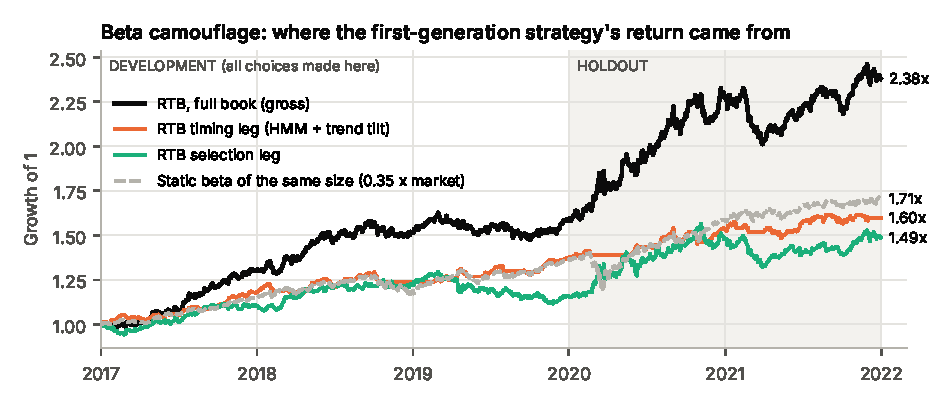
\includegraphics[width=\figw]{fig/fig01.pdf}
\caption{Beta camouflage in the first-generation strategy (RTB). Cumulative gross returns of the full book, of its timing leg (the hidden-Markov and trend tilt of the leg budgets), of its dollar-neutral selection leg, and of a static market exposure equal to the book's average net exposure (0.35). The static exposure finishes above the timing leg, so the overlay delivered the equity premium of the sample and no timing skill.}\label{fig:camouflage}
\end{figure}

\para{The search that followed:} Six audit rounds then looked for a selection alpha, with every new family of hypotheses pre-registered (Table~\ref{tab:ledger}). None of the following passed its pre-registered tests:
\begin{itemize}
  \item new analyst features, an extended library of 18 signals and signal blends
  \item analyst-network spillovers, idiosyncratic momentum and a L\'evy-area lead--lag signal
  \item event-level post-revision drift, analyst-skill weighting and earnings-cycle conditioning
  \item within-analyst relative valuation, normalised revision velocity and dispersion gating
  \item earnings-reaction predictability, and risk-forecasting overlays (Round 6)
\end{itemize}
These rounds taught me two things. Cutting the sample into subsets (event days, analyst histories, cycle phases) lost more power in breadth than it gained in precision, and level signals on target prices carry the price in their denominator. What I needed next was a selection signal with information beyond price momentum, in a construction with no beta.

\begin{table}[t]
\centering\footnotesize
\caption{Research ledger: hypotheses tested before and around the final specification}\label{tab:ledger}
\begin{adjustbox}{max width=\textwidth}\begin{tabular}{p{0.07\textwidth}p{0.43\textwidth}p{0.42\textwidth}}
\toprule
Round & Hypotheses / signals & Outcome\\
\midrule
1 & Fresh-vs-stale consensus wedge, leader/laggard revisions, conviction shock (target change net of price change), post-event drift, bold-revision breadth, peer spillover, quarterly target expiry & None passed the inclusion rule, strongest (conviction shock) IC21 0.034, $p = 0.30$, a 252-session expiry is retained.\\
2 & Library of 18 signals (11 analyst, 7 price), four pre-specified blends, analyst window, rebalancing frequency & LMH is the only signal with FM $t > 2$, blends do not improve, flow window 63 sessions, slower rebalancing dominates.\\
3 & Analyst-network pending revisions (2), idiosyncratic momentum, L\'evy-area lead--lag, upside per unit of volatility, tranche period, volatility scaling & 0 of 10 significant after Holm, network signals wrong-signed, slow tranches, volatility scaling hurts.\\
4 & Eight pre-registered tests: event-level LMH, post-revision drift, confirmed surprise, analyst-skill persistence, two skill-weighted breadths, earnings-phase interaction and gating, overlay decomposition & 0 of 8 after Holm, skill does not persist ($t = -0.22$), event drift reverses in DEV but not in a one-shot holdout test, the overlay is beta.\\
5 & Within-analyst demeaned and ranked target returns, top-pick-weighted breadth, normalised revision velocity (2), dispersion-gated breadth, quiet-day breadth, coverage change, breadth acceleration, linear-rank weights & 0 of 9, within-analyst valuation wrong-signed (IC21 $-0.089$), flow variants duplicate breadth (correlation 0.86--0.96), linear-rank weights worse.\\
6 & Feasibility, persistence-preserving placebos, signal decomposition, earnings-reaction predictability, variance forecasting, risk-based sizing & Reaction predictability null in DEV, analyst dispersion and an earnings-calendar proxy forecast variance beyond GARCH, but sizing by them does not improve the book.\\
\bottomrule
\end{tabular}\end{adjustbox}
\par\smallskip\begin{minipage}{0.95\textwidth}\footnotesize The audit also found and corrected a construction error: a rank-proportional book that was not dollar-neutral (a cross-sectional rank centred at $0.5/N$ instead of zero), which its beta and its random-score placebo exposed.\end{minipage}
\end{table}

\section{First-Mover Flow: signal and construction}\label{sec:fmf}

Let $U_{i,s}$ and $D_{i,s}$ be the numbers of fresh up and down revisions on stock $i$ that become known at session $s$.

\para{Revision-flow signals:} Breadth over the last 63 sessions (one earnings cycle) is
\begin{equation}
B_{i,t}=\frac{\sum_{s=t-62}^{t}\left(U_{i,s}-D_{i,s}\right)}{\sum_{s=t-62}^{t}\left(U_{i,s}+D_{i,s}\right)},\label{eq:breadth}
\end{equation}
defined when there are at least three revisions. Using the sign of a revision rather than its size avoids the heavy tails of revision magnitudes. Event breadth is the same ratio over revisions published on information-event days (five or more ratings on the stock that day). Momentum-orthogonal breadth is the residual from a date-by-date cross-sectional regression of the rank of $B$ on the rank of 6-1 month momentum.

\para{Leader minus herd:} Each fresh revision $r$ on stock $i$ has direction $d_r=\operatorname{sign}\Delta\ln TP$.
\begin{itemize}
  \item $r$ is a \emph{leader} if it is published on an event day, or if no other fresh revision on the stock arrived in the previous ten sessions
  \item $r$ is a \emph{herder} if it is not a leader, arrives 3--15 sessions after the stock's latest event cluster, and points in the cluster's direction
\end{itemize}
Over 126 sessions (two earnings cycles, so that the sparse events cover almost every stock-day),
\begin{equation}
\mathrm{LMH}_{i,t}=\frac{\sum_{r\in W_t} d_r\mathbf 1^{\text{lead}}_r-\sum_{r\in W_t} d_r\mathbf 1^{\text{herd}}_r}{\#\{\text{leaders}\}+\#\{\text{herders}\}},\label{eq:lmh}
\end{equation}
defined when at least three revisions are classified. Every classification uses only revisions known at $t$.

\para{Composite:} The score is the equal-weight average of the four cross-sectional percentile ranks; no weights are estimated \citep{demiguel2009}.

\para{Construction and risk logic:}
\begin{itemize}
  \item \emph{Daily target:} Each session a target book goes long the $k$ highest-ranked names and short the $k$ lowest. Each leg holds half of gross capital, in proportion to $1/\hat\sigma_{i,t}$, where $\hat\sigma_{i,t}$ is a walk-forward GJR-GARCH(1,1)-t volatility forecast \citep{glosten1993}
  \item \emph{Held book:} The book held is the average of the last $f$ targets,
  \begin{equation}
  w_{i,t}=\frac1f\sum_{s=t-f+1}^{t} w^{\text{target}}_{i,s}\label{eq:tranche}
  \end{equation}
  which is the same as holding $f$ overlapping sub-portfolios and opening one each session \citep{jegadeesh1993}. This removes rebalancing-anchor luck (with a single weekly anchor, the development Sharpe ratio of the same signal ranges from 0.34 to 0.71) and spreads execution over time
  \item \emph{Exposure:} The book is dollar-neutral every session. If a mandate wants market exposure, it is a separate, constant and disclosed beta budget $c$ (FMF-B20 for $c=0.2$), never a timed overlay
  \item \emph{Costs:} Net returns are charged 5\,bp per unit of traded notional
\end{itemize}
The construction parameters ($k=4$, $f=42$, inverse-volatility weights) are chosen on DEV from a 30-book grid by bootstrap-median Calmar (Section~\ref{sec:construction}).

\section{Development and holdout results}\label{sec:results}

\subsection{Signal evidence and mechanism}

Table~\ref{tab:signals} and Figure~\ref{fig:mechanism} give the development evidence. All four signals have a positive IC at every horizon. The composite has an IC21 of 0.109 (hit rate 62\%, calibrated $p = 0.045$). LMH has the highest IC21 of the components, is positive in each of the three years, and is the only signal with a Fama-MacBeth $t$-statistic above two after the four price controls. The breadth signals lose significance once momentum is in the regression breadth on its own is largely momentum. The mechanism is directly visible: leader breadth predicts returns, herder breadth predicts reversals, and the difference collects both effects. Information builds over several weeks, with the composite's IC going from 0.026 at one session to 0.109 at 21.

\begin{table}[t]
\centering\small
\caption{Signal evidence development sample (2017-2019)}\label{tab:signals}
\begin{adjustbox}{max width=\textwidth}\begin{tabular}{lrrrrrrrrrr}
\toprule
 & IC5 & IC21 & IC63 & Hit (\%) & $t_{NW}$ & $t_{\text{phase}}$ & $p$ & Holm & Years $>0$ & FM $t$\\
\midrule
breadth\_63 & 0.036 & 0.072 & 0.064 & 61 & 1.50 & 1.16 & 0.127 & 0.30 & 2/3 & 0.21\\
event\_breadth\_63 & 0.033 & 0.085 & 0.082 & 58 & 1.73 & 1.26 & 0.108 & 0.30 & 2/3 & 0.15\\
breadth\_resid\_mom & 0.045 & 0.083 & 0.109 & 56 & 2.03 & 1.45 & 0.078 & 0.30 & 2/3 & 0.36\\
leader\_minus\_herd & 0.049 & 0.095 & 0.104 & 60 & 1.81 & 1.47 & 0.075 & 0.30 & 3/3 & 2.46\\
Composite & 0.053 & 0.109 & 0.114 & 62 & 2.19 & 1.74 & 0.045 & -- & 2/3 & 0.60\\
\quad leaders only & 0.039 & 0.066 & 0.051 & 57 & 1.28 & 1.03 & 0.155 & -- & 2/3 & 0.85\\
\quad herders only & $-0.123$ & $-0.084$ & $-0.148$ & 39 & $-0.78$ & -- & -- & -- & 0/3 & $-0.10$\\
\bottomrule
\end{tabular}\end{adjustbox}
\par\smallskip\begin{minipage}{0.97\textwidth}\footnotesize Mean daily Spearman rank IC with purged forward log returns. $t_{NW}$: Newey-West with 21 lags (shown for continuity it over-rejects). $t_{\text{phase}}$, $p$: calibrated phase-averaged non-overlapping test, one-sided. Holm: adjusted over the four components. FM $t$: Fama--MacBeth $t$ with controls for 12-1 and 6-1 momentum, 1-month reversal and 60-day volatility.\end{minipage}
\end{table}

\begin{figure}[t]
\centering
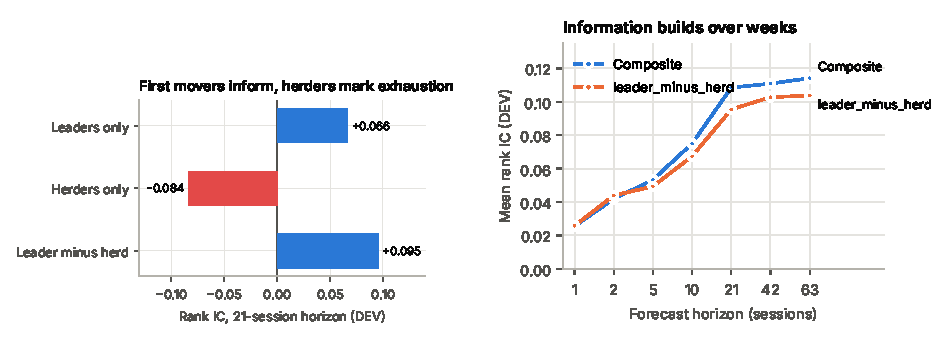
\includegraphics[width=\figw]{fig/fig02.pdf}
\caption{Mechanism and information horizon. Left: rank IC (21 sessions) of breadth from leader revisions only, herder revisions only, and their difference. Right: mean development IC of the composite and of LMH by horizon.}\label{fig:mechanism}
\end{figure}

\subsection{Construction and the price of the search}\label{sec:construction}

Table~\ref{tab:grid} and Figure~\ref{fig:grid} summarise the grid ($k\in\{3,4,5\}$, $f\in\{21,42,63,84,126\}$, equal or inverse-volatility weights). The rule fixed in advance picks $k=4$, $f=42$ and inverse-volatility weights, with a bootstrap-median Calmar of 0.855 against 0.735 for the equal-weight 63-session book. According to the diagnostics this choice is mostly cosmetic. It is also fragile in a literal sense. The rule keeps the lowest-turnover book within 0.02 of the best bootstrap median, and $k=4$ leads $k=5$ by little more than that. On a second machine, where re-estimated GARCH forecasts move the two medians to 0.840 and 0.825, the same rule picks $k=5$, whose 2017--2021 Sharpe ratio is 1.03 instead of 1.13. The book kept here ($k=4$) is the one frozen and pre-registered for the out-of-sample test, and the notebook now holds it fixed and reports when the rule would choose otherwise. The 30 books are near-duplicates (average correlation 0.91) and their in-sample ranking does not persist (PBO 0.945). The level does persist: the in-sample winner's median out-of-sample Sharpe ratio is 0.66. The deflated Sharpe ratio is 0.94 against the grid, 0.38 against the research log of 71 configurations, and 0.18 against all selection (Table~\ref{tab:dsr}). The development Sharpe ratio alone is not enough evidence, and this is why Sections~\ref{sec:toolkit} and~\ref{sec:oos} matter.

\begin{table}[t]
\centering\small
\caption{Development construction grid (top eight books)}\label{tab:grid}
\begin{adjustbox}{max width=\textwidth}\begin{tabular}{rrlrrrrrrr}
\toprule
$k$ & $f$ & Weights & Sharpe & CAGR (\%) & MaxDD (\%) & Calmar & Boot. median & Boot. 5\% & Turnover\\
\midrule
4 & 42 & IV-GJR $\blacklozenge$ & 0.98 & 7.7 & $-9.7$ & 0.79 & 0.85 & $-0.02$ & 2.1\\
5 & 42 & IV-GJR & 0.96 & 6.3 & $-7.7$ & 0.81 & 0.83 & 0.00 & 1.9\\
5 & 63 & IV-GJR & 0.96 & 6.1 & $-7.5$ & 0.81 & 0.81 & 0.00 & 1.4\\
4 & 63 & IV-GJR & 0.95 & 7.3 & $-9.6$ & 0.76 & 0.77 & $-0.05$ & 1.7\\
4 & 42 & EW & 0.91 & 8.1 & $-12.3$ & 0.66 & 0.77 & $-0.08$ & 1.7\\
5 & 63 & EW & 0.93 & 6.7 & $-8.7$ & 0.77 & 0.74 & $-0.06$ & 1.2\\
5 & 42 & EW & 0.88 & 6.4 & $-8.8$ & 0.73 & 0.74 & $-0.07$ & 1.5\\
4 & 21 & IV-GJR & 0.91 & 7.3 & $-10.5$ & 0.69 & 0.74 & $-0.07$ & 3.3\\
4 & 63 & EW (Round 3) & 0.92 & 8.0 & $-11.5$ & 0.69 & 0.73 & $-0.09$ & 1.4\\
\bottomrule
\end{tabular}\end{adjustbox}
\par\smallskip\begin{minipage}{0.97\textwidth}\footnotesize Dollar-neutral, net of 5\,bp. Boot.: Calmar across 1,000 stationary-bootstrap resamples of DEV. Turnover: one-way, times per year. $\blacklozenge$: selected.\end{minipage}
\end{table}

\begin{figure}[t]
\centering
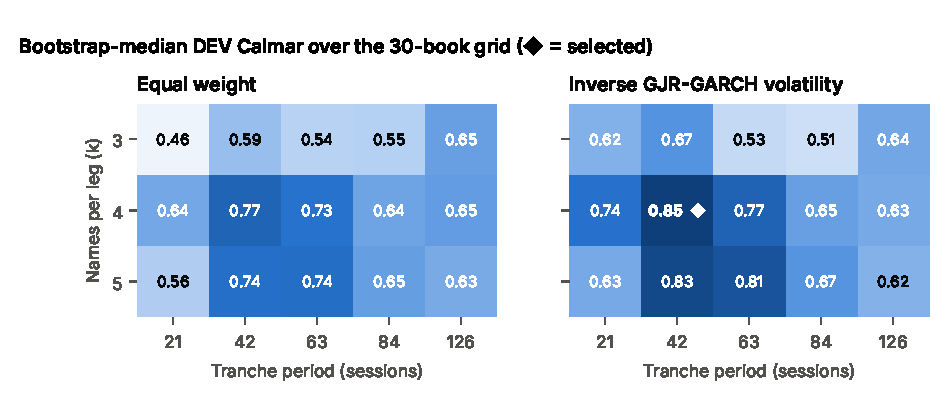
\includegraphics[width=\figw]{fig/fig03.pdf}
\caption{Bootstrap-median development Calmar ratio across the 30-book construction grid.}\label{fig:grid}
\end{figure}

\begin{table}[t]
\centering\small
\caption{Deflated Sharpe ratio of the selected book (development)}\label{tab:dsr}
\begin{adjustbox}{max width=\textwidth}\begin{tabular}{lrrrrr}
\toprule
Trial set & $N_{\text{eff}}$ & $SR_0$ (ann.) & Sharpe (ann.) & PSR(0) & DSR\\
\midrule
Within the 30-book grid & 3.5 & 0.07 & 0.98 & 0.95 & 0.94\\
Audit research log (71 configurations) & 37.2 & 1.15 & 0.98 & 0.95 & 0.38\\
All selection incl.\ pre-log ($\approx$284) & 250.2 & 1.51 & 0.98 & 0.95 & 0.18\\
\bottomrule
\end{tabular}\end{adjustbox}
\par\smallskip\begin{minipage}{0.9\textwidth}\footnotesize $SR_0$: expected maximum annualised Sharpe ratio of $N_{\text{eff}}$ independent null trials. Rows 2--3 use the cross-trial Sharpe dispersion of the research log.\end{minipage}
\end{table}

\subsection{Performance}

Table~\ref{tab:perf} and Figures~\ref{fig:equity}--\ref{fig:drawdown} compare the frozen book with its predecessors and with momentum. After costs FMF-N has Sharpe ratios of 0.98, 1.33 and 1.13 in DEV, the holdout and the full period, with volatility of 9.6\%, a maximum drawdown of $-14.1\%$, a beta of $-0.02$ and a Jensen alpha of 11.9\% a year ($t = 2.32$).
\begin{itemize}
  \item Compared with RTB's selection leg (Calmar 0.36, 0.85 and 0.53, gross of costs), FMF-N about doubles the development Calmar ratio and improves it in every window
  \item Compared with 12-1 momentum built the same way (full-period Sharpe 0.50, Calmar 0.23), FMF-N is more than twice as efficient
  \item Costs matter little: turnover is 2.1--2.7 times a year (10.8 for RTB), and the full-period Sharpe ratio is 1.16 gross and 1.11 at 10\,bp
\end{itemize}

\begin{table}[p]
\centering\small
\caption{Performance of the frozen specification and its predecessors}\label{tab:perf}
\begin{adjustbox}{max width=\textwidth}\begin{tabular}{lrrrrrrrrr}
\toprule
 & CAGR & Vol & Sharpe & MaxDD & Calmar & Beta & $\alpha$ (\%) & $t(\alpha)$ & PSR(0)\\
\midrule
\multicolumn{10}{l}{\emph{Panel A: DEV, 2017--2019}}\\
Revised strategy ($\tau=0$, net 5\,bp) & 7.7 & 7.9 & 0.98 & $-9.7$ & 0.79 & $-0.01$ & 8.2 & 1.82 & 0.95\\
\quad gross of costs & 7.9 & 7.9 & 1.01 & $-9.6$ & 0.82 & $-0.01$ & 8.4 & 1.87 & 0.96\\
\quad net 10\,bp & 7.5 & 7.9 & 0.95 & $-9.7$ & 0.77 & $-0.01$ & 8.0 & 1.77 & 0.95\\
Original selection component (gross) & 5.0 & 8.4 & 0.63 & $-13.9$ & 0.36 & $-0.07$ & 7.5 & 1.78 & 0.86\\
12-1 momentum, same construction (net) & 4.8 & 8.0 & 0.63 & $-11.5$ & 0.42 & 0.07 & 2.9 & 0.51 & 0.86\\
Original full strategy, HMM tilt (gross) & 16.6 & 10.2 & 1.56 & $-9.4$ & 1.77 & 0.20 & 10.2 & 2.46 & 1.00\\
Equal-weight market & 32.7 & 18.9 & 1.59 & $-25.1$ & 1.31 & 1.00 & -- & -- & 1.00\\
\midrule
\multicolumn{10}{l}{\emph{Panel B: Holdout, 2020--2021}}\\
Revised strategy ($\tau=0$, net 5\,bp) & 16.0 & 11.7 & 1.33 & $-14.1$ & 1.14 & $-0.14$ & 21.1 & 2.19 & 0.97\\
\quad gross of costs & 16.3 & 11.7 & 1.35 & $-14.0$ & 1.17 & $-0.14$ & 21.4 & 2.22 & 0.97\\
\quad net 10\,bp & 15.7 & 11.7 & 1.31 & $-14.1$ & 1.11 & $-0.14$ & 20.8 & 2.16 & 0.97\\
Original selection component (gross) & 13.2 & 13.3 & 1.00 & $-15.5$ & 0.85 & $-0.11$ & 17.5 & 2.07 & 0.92\\
12-1 momentum, same construction (net) & 5.2 & 14.2 & 0.43 & $-21.8$ & 0.24 & $-0.17$ & 12.4 & 1.15 & 0.72\\
Original full strategy, HMM tilt (gross) & 22.5 & 14.7 & 1.45 & $-13.6$ & 1.65 & 0.03 & 20.9 & 1.99 & 0.98\\
Equal-weight market & 34.1 & 32.1 & 1.08 & $-38.1$ & 0.89 & 1.00 & -- & -- & 0.93\\
\midrule
\multicolumn{10}{l}{\emph{Panel C: Full period, 2017--2021}}\\
Revised strategy ($\tau=0$, net 5\,bp) & 11.0 & 9.6 & 1.13 & $-14.1$ & 0.78 & $-0.02$ & 11.9 & 2.32 & 0.99\\
\quad gross of costs & 11.2 & 9.6 & 1.16 & $-14.0$ & 0.80 & $-0.02$ & 12.2 & 2.36 & 0.99\\
\quad net 10\,bp & 10.7 & 9.6 & 1.11 & $-14.1$ & 0.76 & $-0.02$ & 11.7 & 2.27 & 0.99\\
Original selection component (gross) & 8.3 & 10.6 & 0.80 & $-15.5$ & 0.53 & $-0.07$ & 10.9 & 2.35 & 0.96\\
12-1 momentum, same construction (net) & 5.0 & 10.9 & 0.50 & $-21.8$ & 0.23 & $-0.02$ & 6.4 & 1.00 & 0.86\\
Original full strategy, HMM tilt (gross) & 19.0 & 12.2 & 1.48 & $-13.6$ & 1.39 & 0.11 & 15.0 & 2.48 & 1.00\\
Equal-weight market & 33.3 & 25.0 & 1.28 & $-38.1$ & 0.87 & 1.00 & -- & -- & 1.00\\
\bottomrule
\end{tabular}\end{adjustbox}
\par\smallskip\begin{minipage}{0.97\textwidth}\footnotesize Percent per year for CAGR, volatility, drawdown and alpha. Beta and Jensen alpha from weekly regressions on the equal-weight market with HAC(4) errors. RTB figures are gross of costs.\end{minipage}
\end{table}

\begin{figure}[t]
\centering
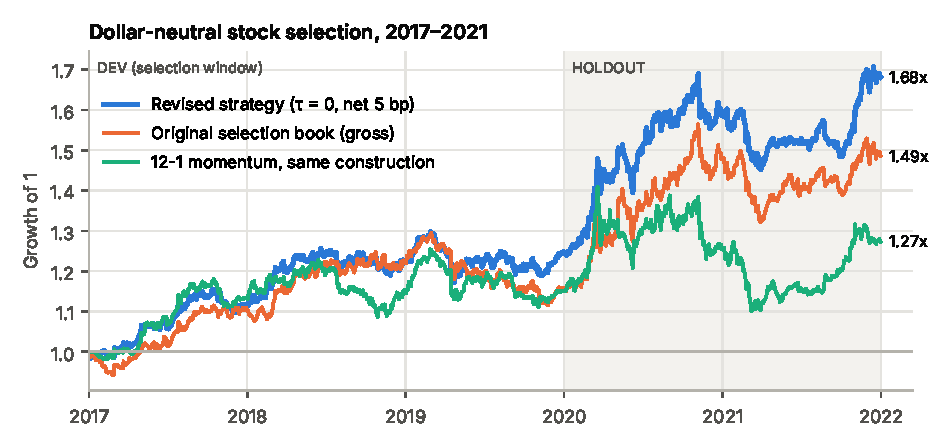
\includegraphics[width=\figw]{fig/fig04.pdf}
\caption{Growth of one unit, 2017--2021. FMF-N and 12-1 momentum are net of 5\,bp per unit traded; RTB's selection leg is gross. Shaded: holdout.}\label{fig:equity}
\end{figure}

\begin{figure}[t]
\centering
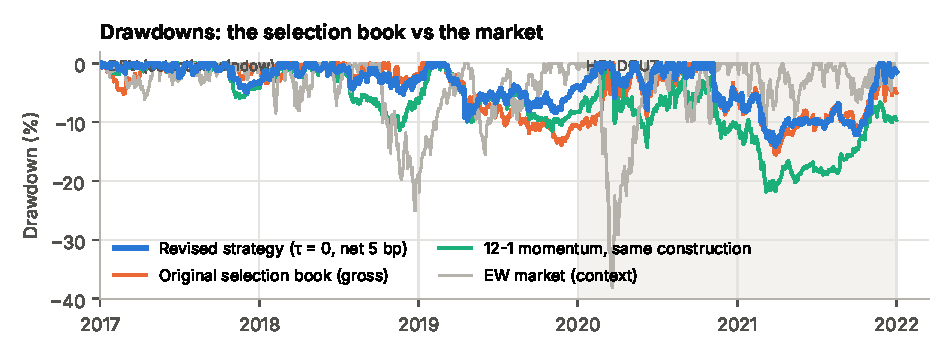
\includegraphics[width=\figw]{fig/fig05.pdf}
\caption{Drawdowns, 2017-2021, with the equal-weight market for context. In February-April 2020 the market's peak-to-trough return was $-38.1\%$, against $-5.8\%$ for FMF-N.}\label{fig:drawdown}
\end{figure}

\subsection{Attribution, placebos and concentration}

Against the market and four factor books built the same way from the price controls, FMF-N loads on 12-1 momentum (0.41) and against reversal ($-0.34$). These explain 0.60 of its variance, and an alpha of 7.4\% a year remains ($t = 2.98$; Table~\ref{tab:attrib}).
\begin{itemize}
  \item \emph{Placebos} (Table~\ref{tab:placebo}, Figure~\ref{fig:placebo}): FMF-N beats IID random scores and stock-label permutations in every window (full period $p = 0.003$ and $0.002$). Against the circular time-shift it passes in the holdout ($p = 0.025$) but not in DEV or over the full period ($p = 0.076$). Some of the edge is therefore which stocks the signal favours
  \item \emph{Leave-one-stock-out} (Table~\ref{tab:loo}, Figure~\ref{fig:loo}): Every rebuild runs the whole pipeline again on nine stocks. The full-period Sharpe ratio is between 0.80 and 1.25 (median 1.06). Without the largest P\&L contributor (stock\_6, about half of P\&L) the Sharpe ratio is 1.08 and the Calmar ratio 0.77. No single name carries the result
\end{itemize}

\begin{table}[t]
\centering\small
\caption{Factor attribution of the weekly book return}\label{tab:attrib}
\begin{adjustbox}{max width=\textwidth}\begin{tabular}{lrrrrrrrr}
\toprule
Window & $\alpha$ (\%) & $t(\alpha)$ & Market & Mom 12-1 & Mom 6-1 & Rev 1m & Low vol & $R^2$\\
\midrule
DEV & 6.0 & 2.33 & $-0.03$ & 0.67 & 0.08 & $-0.34$ & 0.08 & 0.67\\
Holdout & 12.3 & 2.03 & $-0.05$ & 0.20 & 0.26 & $-0.53$ & $-0.07$ & 0.63\\
Full & 7.4 & 2.98 & 0.02 & 0.41 & 0.25 & $-0.34$ & 0.05 & 0.60\\
\bottomrule
\end{tabular}\end{adjustbox}
\par\smallskip\begin{minipage}{0.9\textwidth}\footnotesize OLS on non-overlapping weekly returns, HAC(4) errors, factor books built with the strategy's construction.\end{minipage}
\end{table}

\begin{table}[t]
\centering\small
\caption{Placebo tests through the identical construction}\label{tab:placebo}
\begin{adjustbox}{max width=\textwidth}\begin{tabular}{llrrrrrrr}
\toprule
Window & Null & Draws & Sharpe & Null 95th & $p$ & Calmar & Null 95th & $p$\\
\midrule
DEV & IID random scores & 300 & 0.98 & 0.72 & 0.033 & 0.79 & 0.59 & 0.033\\
 & Stock-label permutation & 500 & 0.98 & 0.75 & 0.022 & 0.79 & 0.60 & 0.026\\
 & Circular time-shift & 315 & 0.98 & 1.39 & 0.146 & 0.79 & 1.52 & 0.146\\
Holdout & IID random scores & 300 & 1.33 & 0.80 & 0.010 & 1.14 & 0.69 & 0.017\\
 & Stock-label permutation & 500 & 1.33 & 0.98 & 0.016 & 1.14 & 1.06 & 0.044\\
 & Circular time-shift & 315 & 1.33 & 1.24 & 0.025 & 1.14 & 1.19 & 0.060\\
Full & IID random scores & 300 & 1.13 & 0.44 & 0.003 & 0.78 & 0.22 & 0.003\\
 & Stock-label permutation & 500 & 1.13 & 0.56 & 0.002 & 0.78 & 0.37 & 0.004\\
 & Circular time-shift & 315 & 1.13 & 1.21 & 0.076 & 0.78 & 1.05 & 0.076\\
\bottomrule
\end{tabular}\end{adjustbox}
\par\smallskip\footnotesize $p = (1+\#\{\text{null}\ge\text{observed}\})/(1+\text{draws})$.
\end{table}

\begin{figure}[t]
\centering
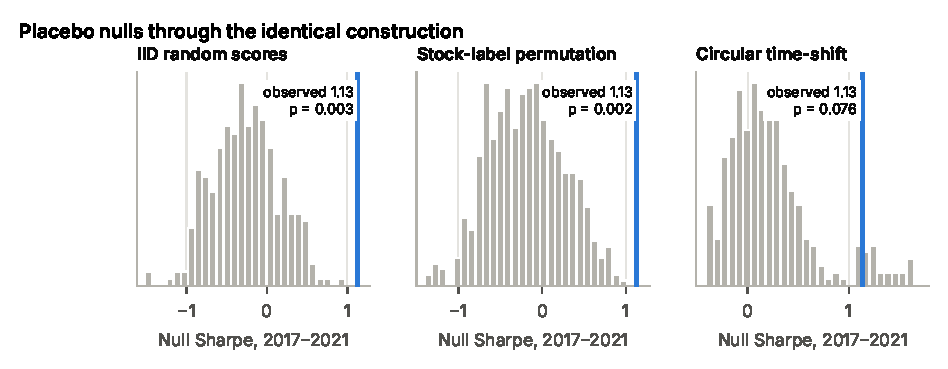
\includegraphics[width=\figw]{fig/fig06.pdf}
\caption{Full-period Sharpe ratios under the three placebo nulls; the line marks the observed value.}\label{fig:placebo}
\end{figure}

\begin{table}[t]
\centering\small
\caption{Full leave-one-stock-out rebuilds}\label{tab:loo}
\begin{adjustbox}{max width=\textwidth}\begin{tabular}{lrrrrrrrrr}
\toprule
 & \multicolumn{3}{c}{Sharpe} & \multicolumn{3}{c}{Calmar} & MaxDD & $\alpha$ & $t(\alpha)$\\
\cmidrule(lr){2-4}\cmidrule(lr){5-7}
Universe & DEV & Hold. & Full & DEV & Hold. & Full & Full (\%) & Full (\%) & Full\\
\midrule
All ten stocks & 0.98 & 1.33 & 1.13 & 0.79 & 1.14 & 0.78 & $-14.1$ & 11.9 & 2.32\\
without stock\_1 & 1.14 & 1.14 & 1.12 & 1.00 & 0.92 & 0.75 & $-14.7$ & 12.4 & 2.39\\
without stock\_2 & 0.58 & 1.10 & 0.81 & 0.47 & 0.96 & 0.62 & $-10.7$ & 5.5 & 1.37\\
without stock\_3 & 0.78 & 0.91 & 0.83 & 0.63 & 0.65 & 0.49 & $-14.3$ & 9.0 & 2.03\\
without stock\_4 & 0.90 & 0.72 & 0.80 & 0.77 & 0.50 & 0.46 & $-15.8$ & 8.6 & 1.72\\
without stock\_5 & 1.03 & 1.53 & 1.25 & 0.78 & 1.56 & 1.05 & $-11.4$ & 13.3 & 2.73\\
without stock\_6 & 0.87 & 1.34 & 1.08 & 0.66 & 1.18 & 0.77 & $-13.8$ & 10.6 & 1.98\\
without stock\_7 & 1.03 & 1.32 & 1.15 & 0.80 & 1.17 & 0.80 & $-14.1$ & 12.9 & 2.42\\
without stock\_8 & 0.80 & 1.27 & 1.02 & 0.63 & 1.16 & 0.73 & $-12.8$ & 10.4 & 1.99\\
without stock\_9 & 0.86 & 1.47 & 1.14 & 0.66 & 1.39 & 0.84 & $-12.5$ & 11.1 & 2.33\\
without stock\_10 & 0.98 & 1.15 & 1.04 & 1.23 & 0.91 & 0.65 & $-14.7$ & 10.3 & 2.13\\
\bottomrule
\end{tabular}\end{adjustbox}
\par\smallskip\begin{minipage}{0.95\textwidth}\footnotesize Each row repeats cleaning, calendar, snapshot, features, cross-sectional ranks, composite and allocation without one stock. GARCH forecasts are univariate and so do not change.\end{minipage}
\end{table}

\begin{figure}[t]
\centering
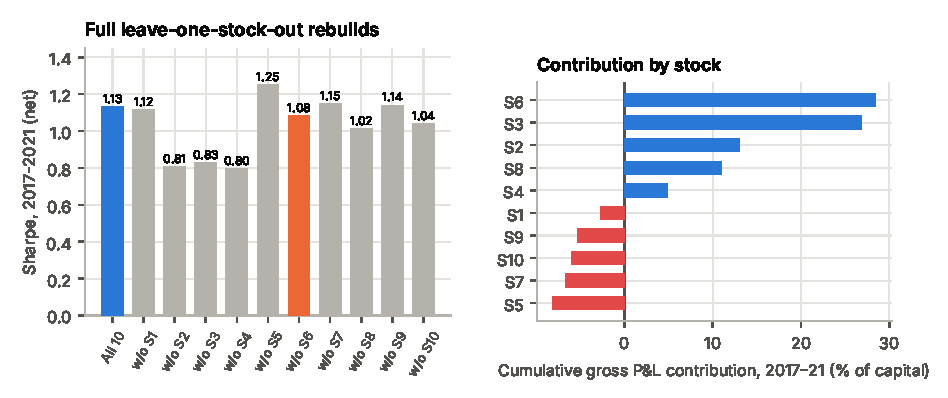
\includegraphics[width=\figw]{fig/fig07.pdf}
\caption{Left: full-period Sharpe ratio of the ten leave-one-stock-out rebuilds (orange: without the largest contributor). Right: cumulative gross P\&L by stock.}\label{fig:loo}
\end{figure}

\section{First-Mover Flow versus the institutional toolkit}\label{sec:toolkit}

A selection signal has value for a portfolio manager only when it adds something the standard toolkit lacks. I build 13 cross-sectional comparables (Appendix~\ref{app:defs}) with FMF-N's construction, so that any difference comes from the signal, and add three allocations. The comparables cover the price factors, the sell-side signals in common use and two multi-factor blends.

\para{League table:} Of the 14 cross-sectional books, FMF-N has the highest full-period Sharpe (1.13) and Calmar (0.78) ratios (Table~\ref{tab:league}, Figure~\ref{fig:league}). Next are classic revision breadth (0.92 and 0.58), itself one of FMF-N's components, and the momentum + revisions blend (0.87 and 0.49). Plain 12-1 momentum gets 0.50 and 0.23. Betting-against-beta, low dispersion and reversal lose money in this universe.

\para{Where the toolkit fails:} Figure~\ref{fig:episodes} and Table~\ref{tab:episodes} cover five named episodes.
\begin{itemize}
  \item \emph{COVID crash:} Market $-35.5\%$, betting-against-beta $-15.2\%$, reversal $-7.7\%$; FMF-N $+12.0\%$.
  \item \emph{Vaccine rotation (November 2020):} In this momentum crash FMF-N returned $-5.8\%$, against $-8.2\%$ for both 12-1 and residual momentum.
  \item \emph{Feb-Mar 2021 growth sell-off:} FMF-N's worst episode ($-7.1\%$) was milder than for 12-1 momentum ($-10.5\%$) and time-series momentum ($-12.1\%$).
\end{itemize}

\para{Spanning:} Regressed on the market and all 13 comparables, FMF-N's alpha falls to 1.8\% ($t = 1.46$, $R^2 = 0.92$; Table~\ref{tab:spanning}). This test is circular, since two comparables contain FMF-N's components. Against the market and the 11 comparables not built from its components the alpha is 6.1\% a year ($t = 2.51$) over 2017--2021 and 7.5\% ($t = 3.86$) in DEV.

\begin{table}[t]
\centering\footnotesize
\caption{FMF-N and institutional comparables, identical construction (net of 5\,bp)}\label{tab:league}
\begin{adjustbox}{max width=\textwidth}\begin{tabular}{lrrrrrrrrr}
\toprule
 & \multicolumn{3}{c}{Sharpe} & \multicolumn{3}{c}{Calmar} & MaxDD & Beta & Corr.\\
\cmidrule(lr){2-4}\cmidrule(lr){5-7}
 & DEV & Hold. & Full & DEV & Hold. & Full & Full (\%) & Full & FMF-N\\
\midrule
FMF-N (this paper) & 0.98 & 1.33 & 1.13 & 0.79 & 1.14 & 0.78 & $-14.1$ & $-0.02$ & 1.00\\
Revision breadth (classic) & 0.57 & 1.28 & 0.92 & 0.38 & 1.08 & 0.58 & $-15.5$ & $-0.02$ & 0.95\\
Momentum + revisions blend & 0.78 & 1.01 & 0.87 & 0.52 & 0.73 & 0.49 & $-18.5$ & $-0.01$ & 0.90\\
Multi-factor: mom + low vol + reversal & 0.88 & 0.80 & 0.81 & 0.71 & 0.52 & 0.42 & $-14.3$ & $-0.09$ & 0.44\\
Low volatility (60d) & 0.37 & 0.80 & 0.56 & 0.21 & 1.18 & 0.37 & $-13.6$ & $-0.10$ & 0.04\\
12-1 momentum (Jegadeesh-Titman) & 0.63 & 0.43 & 0.50 & 0.42 & 0.24 & 0.23 & $-21.8$ & $-0.02$ & 0.71\\
Target-price upside (consensus) & 0.47 & 0.29 & 0.38 & 0.37 & 0.24 & 0.24 & $-12.1$ & 0.04 & $-0.38$\\
52-week-high proximity & $-0.36$ & 1.06 & 0.37 & $-0.16$ & 0.75 & 0.17 & $-18.2$ & $-0.09$ & 0.73\\
Target-price momentum (63d) & $-0.36$ & 0.68 & 0.19 & $-0.15$ & 0.44 & 0.07 & $-20.4$ & $-0.08$ & 0.71\\
Residual momentum (Blitz et al.) & 0.42 & 0.00 & 0.17 & 0.24 & $-0.04$ & 0.05 & $-24.1$ & $-0.06$ & 0.64\\
6-1 momentum & $-0.51$ & 0.55 & 0.06 & $-0.16$ & 0.32 & 0.00 & $-24.8$ & $-0.04$ & 0.67\\
Betting-against-beta (low beta) & $-0.28$ & 0.00 & $-0.15$ & $-0.17$ & $-0.05$ & $-0.07$ & $-32.2$ & 0.01 & 0.10\\
Short-term reversal (1m) & 0.25 & $-0.69$ & $-0.24$ & 0.16 & $-0.33$ & $-0.09$ & $-18.7$ & 0.04 & $-0.51$\\
Low analyst dispersion & $-0.36$ & $-0.74$ & $-0.53$ & $-0.19$ & $-0.50$ & $-0.20$ & $-27.7$ & $-0.13$ & $-0.15$\\
\midrule
\multicolumn{10}{l}{\emph{Allocation benchmarks}}\\
Equal-weight long-only (market) & 1.59 & 1.08 & 1.28 & 1.31 & 0.89 & 0.87 & $-38.1$ & 1.00 & $-0.02$\\
Inverse-vol long-only (naive risk parity) & 1.67 & 1.17 & 1.35 & 1.37 & 0.99 & 0.92 & $-37.2$ & 0.96 & $-0.01$\\
Time-series momentum 12-1 (CTA-style) & 0.89 & 0.86 & 0.86 & 0.57 & 0.89 & 0.54 & $-30.2$ & 0.61 & 0.29\\
RTB: original regime-timed breadth (gross) & 1.56 & 1.45 & 1.48 & 1.77 & 1.65 & 1.39 & $-13.6$ & 0.11 & 0.63\\
FMF-B20: FMF + explicit 0.2 beta budget & 1.56 & 1.73 & 1.62 & 1.82 & 2.17 & 1.66 & $-10.8$ & 0.17 & 0.89\\
\bottomrule
\end{tabular}\end{adjustbox}
\par\smallskip\begin{minipage}{0.97\textwidth}\footnotesize Cross-sectional comparables: top/bottom four, inverse-GJR weights, 42-session tranches, $\tau=0$, net of 5\,bp. Allocation benchmarks in their natural form. RTB gross; FMF-B20 adds a constant 0.2 beta budget to FMF-N.\end{minipage}
\end{table}

\begin{table}[t]
\centering\footnotesize
\caption{Named episodes: cumulative returns (\%)}\label{tab:episodes}
\begin{adjustbox}{max width=\textwidth}\begin{tabular}{lrrrrr}
\toprule
 & Q4-2018 & COVID crash & COVID rebound & Vaccine rotation & Growth sell-off\\
 & 10/03--12/24/18 & 02/19--03/23/20 & 03/24--06/08/20 & 11/06--11/30/20 & 02/12--03/08/21\\
\midrule
FMF-N & $-0.8$ & 12.0 & $-4.0$ & $-5.8$ & $-7.1$\\
12-1 momentum (Jegadeesh-Titman) & $-0.6$ & 12.2 & $-9.8$ & $-8.2$ & $-10.5$\\
Residual momentum (Blitz et al.) & 5.3 & 8.3 & $-11.1$ & $-8.2$ & $-10.4$\\
Low volatility (60d) & 2.6 & $-0.6$ & 2.8 & 2.8 & 1.2\\
Betting-against-beta (low beta) & 1.3 & $-15.2$ & 3.0 & $-1.0$ & $-1.7$\\
Short-term reversal (1m) & 1.9 & $-7.7$ & 2.4 & 4.0 & 1.1\\
Target-price upside (consensus) & 3.1 & $-3.7$ & 6.3 & 7.3 & 1.7\\
Revision breadth (classic) & $-1.7$ & 10.2 & $-2.3$ & $-7.4$ & $-6.1$\\
Multi-factor: mom + low vol + reversal & 4.2 & 6.0 & $-5.8$ & $-0.7$ & $-4.7$\\
Time-series momentum 12-1 (CTA-style) & $-23.3$ & $-18.9$ & 18.5 & $-3.5$ & $-12.1$\\
Equal-weight long-only (market) & $-24.8$ & $-35.5$ & 60.9 & 6.9 & $-9.4$\\
RTB: original regime-timed breadth & $-4.1$ & 11.9 & $-1.1$ & $-5.5$ & $-9.2$\\
\bottomrule
\end{tabular}\end{adjustbox}
\end{table}

\begin{figure}[t]
\centering
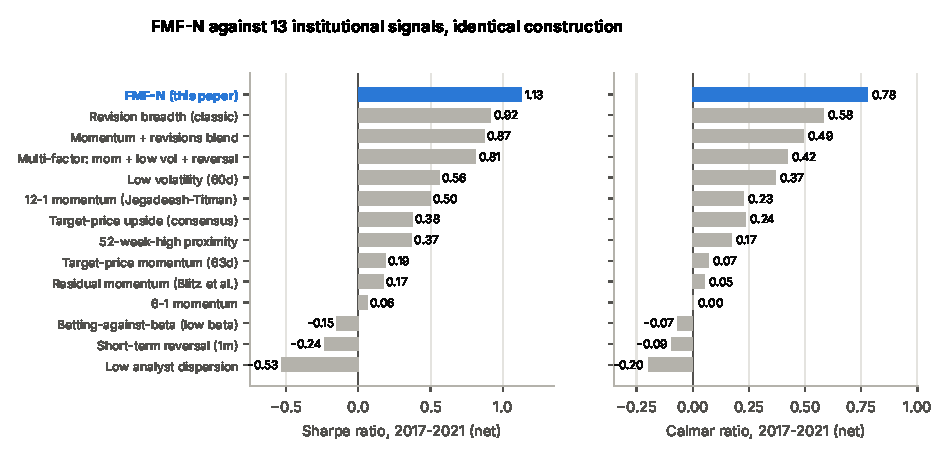
\includegraphics[width=\figw]{fig/fig08.pdf}
\caption{Full-period Sharpe and Calmar ratios of FMF-N and 13 institutional signals built through the identical construction.}\label{fig:league}
\end{figure}

\begin{figure}[t]
\centering
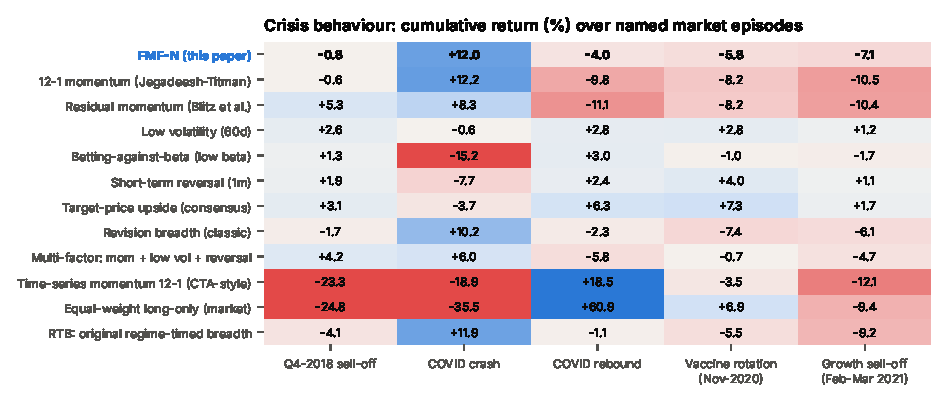
\includegraphics[width=\figw]{fig/fig09.pdf}
\caption{Cumulative return over named market episodes (blue: gain, red: loss).}\label{fig:episodes}
\end{figure}

\para{Blending:} Blended 50/50 with FMF-N, 16 of 18 comparables get a higher Sharpe ratio and 16 of 18 a higher Calmar ratio (Figure~\ref{fig:blend}). The two that do not are the books which already hold market beta (RTB and FMF-B20); their Calmar ratios come from the bull market

\para{Tranches and native form:} Slow tranches suit slow analyst-flow signals (classic breadth: full-period Sharpe 0.92 in tranches, 0.52 in native monthly form) but not every price signal (12-1 momentum: 0.74 native, 0.50 in tranches)

\begin{table}[t]
\centering\small
\caption{Spanning regressions of the weekly FMF-N return}\label{tab:spanning}
\begin{adjustbox}{max width=\textwidth}\begin{tabular}{llrrr}
\toprule
Regressors & Window & $\alpha$ (\% p.a.) & $t(\alpha)$ & $R^2$\\
\midrule
Market + all 13 comparables & DEV & 2.4 & 2.19 & 0.95\\
 & Holdout & 1.2 & 0.50 & 0.93\\
 & Full & 1.8 & 1.46 & 0.92\\
Market + 11 comparables not built from FMF components & DEV & 7.5 & 3.86 & 0.77\\
 & Holdout & 6.4 & 1.02 & 0.69\\
 & Full & 6.1 & 2.51 & 0.69\\
\bottomrule
\end{tabular}\end{adjustbox}
\par\smallskip\begin{minipage}{0.9\textwidth}\footnotesize OLS on non-overlapping weekly returns, HAC(4) errors. The first panel includes classic breadth and the momentum + revisions blend, both built from FMF-N's components.\end{minipage}
\end{table}

\begin{figure}[t]
\centering
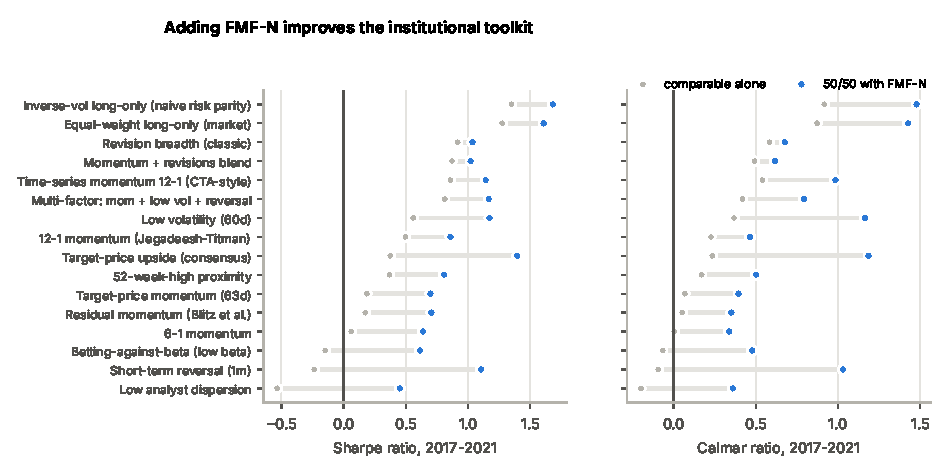
\includegraphics[width=\figw]{fig/fig10.pdf}
\caption{Full-period Sharpe and Calmar ratios of each comparable alone (grey) and blended 50/50 with FMF-N (blue).}\label{fig:blend}
\end{figure}

\section{Out of sample: a never-seen period}\label{sec:oos}

\para{Protocol:} The transfer rules were written to a file and hashed before any return on the new universe was computed (Appendix~\ref{app:prereg}). Only structural information was looked at beforehand: file layout, date range, rating counts, the cleaning log and signal coverage.
\begin{itemize}
  \item \emph{Frozen from development:} signals, LMH parameters, tranche period, allocator, costs and data rules
  \item \emph{Names per leg:} the development choice of 4 names out of 10 becomes a leg fraction of 0.4 of the names with a valid score each session, $k_t=\max(2,\lfloor 0.4N_t\rfloor)$ (primary). The literal $k=4$ is the secondary rule
  \item \emph{Evaluation window:} from 2024-01-05 to 2026-08-05 (647 sessions), after a 252-session warm-up
\end{itemize}
Nothing was changed afterwards.

\para{Results:} The primary book has a net Sharpe ratio of 1.05, a CAGR of 10.5\% at 10.0\% volatility, a maximum drawdown of $-8.0\%$ and a Calmar ratio of 1.32 (Table~\ref{tab:oos}, Figure~\ref{fig:oos}). Beta is $-0.02$ and the Jensen alpha 11.4\% a year ($t = 2.04$). The PSR is 0.95, and deflating over the two pre-registered variants leaves it at that level because the two are highly correlated. Both halves of the window are positive (Sharpe 1.44 and 0.88). The literal $k=4$ rule, four names per leg out of about 19, does worse (Sharpe 0.70, Calmar 0.72), in a wider universe breadth should grow with the universe, which is what the pre-registration says

\begin{table}[t]
\centering\footnotesize
\caption{Out of sample: frozen FMF-N over the never-seen period (net of 5\,bp)}\label{tab:oos}
\setlength{\tabcolsep}{4pt}
\begin{adjustbox}{max width=\textwidth}\begin{tabular}{lrrrrrrrrrrr}
\toprule
 & CAGR & Vol & Sharpe & MaxDD & Calmar & Beta & $\alpha$ & $t(\alpha)$ & PSR & Sharpe H1 & Sharpe H2\\
\midrule
FMF-N, primary (leg fraction 0.4) & 10.5 & 10.0 & 1.05 & $-8.0$ & 1.32 & $-0.02$ & 11.4 & 2.04 & 0.95 & 1.44 & 0.88\\
FMF-N, secondary ($k=4$) & 7.3 & 10.9 & 0.70 & $-10.2$ & 0.72 & $-0.04$ & 8.8 & 1.48 & 0.87 & 0.94 & 0.64\\
FMF-B20, beta budget 0.2 (exploratory)$^\dagger$ & 15.9 & 10.3 & 1.49 & $-6.5$ & 2.43 & 0.16 & 11.8 & 2.09 & 0.99 & 1.73 & 1.44\\
Equal-weight market (30 stocks) & 23.6 & 20.4 & 1.14 & $-25.3$ & 0.94 & 1.00 & -- & -- & 0.97 & 0.28 & 2.35\\
\bottomrule
\end{tabular}\end{adjustbox}
\par\smallskip\begin{minipage}{0.97\textwidth}\footnotesize Evaluation window 2024-01-05 to 2026-08-05. Percent per year for CAGR, volatility, drawdown and alpha. H1 and H2: halves of the window. $^\dagger$ Not in the pre-registration; the budget was fixed in development. Reported for information and used in no test.\end{minipage}
\end{table}

\para{The new signal replicates:} Out of sample LMH has an IC21 of 0.096 (one-sided $p = 0.042$), almost the development value (0.095; Table~\ref{tab:oos_signals}, Figure~\ref{fig:oos_ic}). Breadth (0.051) and the composite (0.073, $p = 0.065$) are positive. Event breadth is negative, but it covers only 26\% of stock-days: clusters of five same-day ratings are rare with 13 analysts per stock

\para{Against the toolkit, out of sample:} FMF-N is 2nd of 14 cross-sectional books on both Sharpe and Calmar (Table~\ref{tab:oos_league}, Figure~\ref{fig:oos_ic}). Only target-price momentum is ahead in this period (1.14 and 1.44). A 50/50 blend with FMF-N raises the Sharpe and Calmar ratios of all 16 comparables. The market and CTA-style trend have high Sharpe ratios in this bull period, with betas of 1.00 and 0.43 and drawdowns of $-25.3\%$ and $-10.8\%$

\para{Placebos and attribution:} The book beats IID random scores ($p = 0.027$) and is borderline against the stock-label permutation ($p = 0.056$). That figure comes from the notebook, whose permutations are unrestricted, so a few stocks keep their own signal in each draw; with derangements, as in development and in the package, $p = 0.046$. Against the circular time-shift it is not significant ($p = 0.226$), as in development (Table~\ref{tab:oos_placebo}). After the market and the four price-control books, alpha is 7.3\% ($t = 1.79$, $R^2 = 0.47$). With a 2.6-year window this is one more sample and not a proof. It is, however, the first sample never used for any choice, and both signatures of the method come back in it: zero beta with positive alpha, and LMH predicting returns

\begin{figure}[t]
\centering
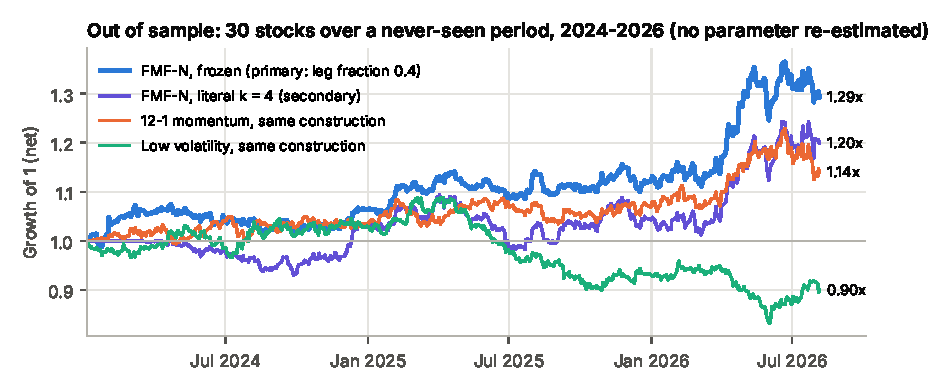
\includegraphics[width=\figw]{fig/fig11.pdf}
\caption{Growth of one unit over the never-seen period, frozen specification, net of 5\,bp.}\label{fig:oos}
\end{figure}

\begin{table}[t]
\centering\small
\caption{Out-of-sample signal evidence (labels inside the evaluation window)}\label{tab:oos_signals}
\begin{adjustbox}{max width=\textwidth}\begin{tabular}{lrrrrr}
\toprule
 & IC21 & $t_{\text{phase}}$ & $p$ & Hit (\%) & Coverage (\%)\\
\midrule
breadth\_63 & 0.051 & 0.98 & 0.168 & 58 & 47\\
event\_breadth\_63 & $-0.041$ & $-0.49$ & 0.685 & 46 & 26\\
breadth\_resid\_mom & 0.020 & 0.39 & 0.351 & 52 & 46\\
leader\_minus\_herd & 0.096 & 1.80 & 0.042 & 64 & 53\\
Composite & 0.073 & 1.56 & 0.065 & 58 & 59\\
\quad leaders only & 0.087 & 1.70 & 0.050 & 61 & 74\\
\bottomrule
\end{tabular}\end{adjustbox}
\end{table}

\begin{figure}[t]
\centering
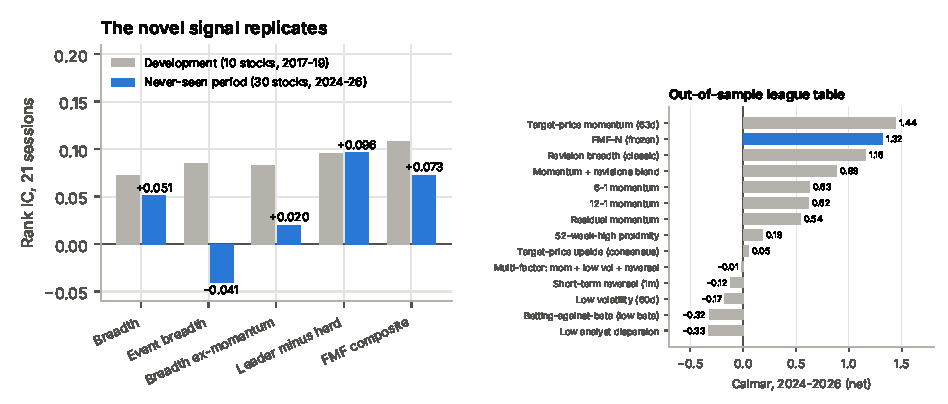
\includegraphics[width=\figw]{fig/fig12.pdf}
\caption{Left: rank IC (21 sessions) of each signal in development and over the never-seen period. Right: out-of-sample Calmar ratios of FMF-N and the cross-sectional comparables.}\label{fig:oos_ic}
\end{figure}

\begin{table}[t]
\centering\small
\caption{Out-of-sample placebo tests}\label{tab:oos_placebo}
\begin{adjustbox}{max width=\textwidth}\begin{tabular}{lrrrrr}
\toprule
Null & Draws & Sharpe & Null median & Null 95th & $p$\\
\midrule
IID random scores & 300 & 1.05 & $-0.26$ & 0.87 & 0.027\\
Stock-label permutation & 500 & 1.05 & $-0.01$ & 1.07 & 0.056\\
Circular time-shift & 216 & 1.05 & 0.09 & 2.17 & 0.226\\
\bottomrule
\end{tabular}\end{adjustbox}
\end{table}

\begin{table}[t]
\centering\footnotesize
\caption{Out of sample: FMF-N and institutional comparables}\label{tab:oos_league}
\begin{adjustbox}{max width=\textwidth}\begin{tabular}{lrrrrrrr}
\toprule
 & & & & & & \multicolumn{2}{c}{50/50 with FMF-N}\\
\cmidrule(lr){7-8}
 & Sharpe & Calmar & MaxDD (\%) & Beta & Corr.\ FMF-N & Sharpe & Calmar\\
\midrule
Time-series momentum 12-1 (CTA-style) & 1.30 & 1.62 & $-10.8$ & 0.43 & 0.33 & 1.45 & 1.86\\
Inverse-vol long-only (naive risk parity) & 1.23 & 1.01 & $-22.5$ & 0.88 & $-0.10$ & 1.66 & 1.56\\
Equal-weight long-only (market) & 1.14 & 0.94 & $-25.3$ & 1.00 & $-0.09$ & 1.54 & 1.41\\
Target-price momentum (63d) & 1.14 & 1.44 & $-7.5$ & 0.04 & 0.67 & 1.19 & 1.76\\
FMF-N (frozen) & 1.05 & 1.32 & $-8.0$ & $-0.02$ & 1.00 & -- & --\\
Revision breadth (classic) & 0.98 & 1.16 & $-8.7$ & $-0.01$ & 0.87 & 1.05 & 1.24\\
Momentum + revisions blend & 0.79 & 0.89 & $-8.2$ & 0.08 & 0.66 & 1.01 & 1.26\\
12-1 momentum (Jegadeesh-Titman) & 0.60 & 0.62 & $-8.5$ & 0.09 & 0.61 & 0.92 & 1.10\\
6-1 momentum & 0.56 & 0.63 & $-7.2$ & 0.04 & 0.63 & 0.91 & 1.09\\
Residual momentum (Blitz et al.) & 0.56 & 0.54 & $-7.9$ & 0.02 & 0.66 & 0.91 & 1.08\\
52-week-high proximity & 0.31 & 0.19 & $-12.0$ & $-0.09$ & 0.66 & 0.79 & 0.81\\
Target-price upside (consensus) & 0.11 & 0.05 & $-11.7$ & 0.05 & $-0.47$ & 1.19 & 1.50\\
Multi-factor: mom + low vol + reversal & 0.00 & $-0.01$ & $-14.3$ & $-0.13$ & 0.39 & 0.77 & 0.71\\
Short-term reversal (1m) & $-0.14$ & $-0.12$ & $-7.9$ & 0.00 & $-0.41$ & 1.05 & 1.07\\
Low volatility (60d) & $-0.39$ & $-0.17$ & $-23.5$ & $-0.26$ & 0.12 & 0.47 & 0.31\\
Low analyst dispersion & $-0.89$ & $-0.33$ & $-25.5$ & $-0.28$ & $-0.13$ & 0.17 & 0.10\\
Betting-against-beta (low beta) & $-0.94$ & $-0.32$ & $-34.3$ & $-0.33$ & $-0.19$ & $-0.04$ & $-0.04$\\
\bottomrule
\end{tabular}\end{adjustbox}
\end{table}

\para{Is the result carried by the ten development names?} Ten of the thirty names are the development stocks, seen again two years later. A post-hoc split, outside the pre-registration, re-runs the frozen specification on each part with the same GARCH forecasts. On the twenty names never used in development the book has a net Sharpe ratio of 0.80, a Calmar ratio of 0.98 and a maximum drawdown of $-9.2\%$, and LMH keeps its information coefficient (IC21 0.105, one-sided $p = 0.058$). The ten development names alone earn 0.31, with LMH near zero (0.022), but with sparse broker coverage a valid cross-section exists for only part of the window. The result is not a re-run of known names, and the new names, if anything, carry it. How the twenty names were chosen is another matter. They are today's large caps, a selection that already knows which companies grew large. A dollar-neutral book is exposed to this choice only through the spread between its legs, and the static tilt towards particular names loses money out of sample (Section~\ref{sec:identity})

\para{An exploratory check of the beta budget:} The pre-registration lists only the two market-neutral variants, so the beta-budget variant is reported apart and is used in no test. With the same scores and leg fraction and the budget $c=0.2$ fixed in development, FMF-B20 has a Sharpe ratio of 1.49, a Calmar ratio of 2.43 and a maximum drawdown of $-6.5\%$ at a beta of 0.16. The Jensen alpha does not change (11.8\% a year, $t = 2.09$), as expected, because the budget adds market return and no skill. In a bull window this is the expected direction. In a falling market the budget costs about $c$ times the market's loss, and for this reason it is a disclosed constant and not a timed bet

\section{Attacking the result: nine objections and what the data say}\label{sec:objections}

Throughout the research we raised nine objections to this ten-stock backtest that are tested here (Table~\ref{tab:objections}). Tests on the strategy use the frozen specification. Tests on the research process use the full family of reasonable specifications. The code is \texttt{scripts/reproduce\_audit.py} in the repository and Block 17 of the notebook.

\begin{table}[t]
\centering\scriptsize
\caption{Anticipated objections, the test applied and the verdict}\label{tab:objections}
\begin{adjustbox}{max width=\textwidth}\begin{tabular}{p{0.24\textwidth}p{0.29\textwidth}p{0.39\textwidth}}
\toprule
Objection & Test & Result\\
\midrule
1. The universe was chosen with hindsight, the book is long the later winners. & Lo (2008) decomposition, causal static and timing books, partial pooling of per-stock P\&L & The timing book carries the edge (Sharpe 1.04, $t = 2.41$, never-seen 1.33, $t = 2.21$). The static tilt is insignificant and negative out of sample.\\
2. Execution at the signal close and free shorting are unrealistic. & 0-2 session delay $\times$ 0-200\,bp borrow $\times$ 0-30\,bp costs, breakeven cost & Sharpe 0.96 (0.89 never-seen) in the harshest cell, breakeven cost 234\,bp per unit traded.\\
3. Overlapping tranches smooth P\&L and inflate the Sharpe ratio. & Lo (2002) autocorrelation-adjusted Sharpe & 1.06 and 1.06, first-order autocorrelation 0.04.\\
4. Zero average beta hides crash beta. & Up- and down-market betas, worst market weeks & Down-market beta $-0.07$ ($t = -1.24$), positive mean return in the worst market decile.\\
5. The parameters were chosen to make it work. & Multiverse of $\approx$300 specifications, SPA, PBO, selection-free ensemble & 99\% (97\%) of specifications earn a positive Sharpe, the ensemble earns 0.92 ($t = 1.97$) and 0.86.\\
6. Beating the toolkit is cherry-picking. & Romano-Wolf step-down against 16 books, reverse SPA & No comparable beats FMF-N (SPA $p = 0.86$, 0.86), FMF-N significantly beats 2 books after FWER control in sample.\\
7. The new signal adds nothing to classic breadth. & FMF-N vs the same book without LMH, pooled across samples & $+0.28$ Sharpe ($p = 0.028$) in sample, $+0.30$ out of sample, $P(\text{gain}>0) = 0.94$ pooled.\\
8. Ten stocks and a few years prove nothing. & Bayesian Sharpe under sceptical priors, random-effects meta-analysis, empirical-Bayes shrinkage, Bayes factors, power & $P(IC>0$ in the next universe$) = 0.96$, pooled IC 0.105, Stouffer $p = 0.0022$, the 18-signal search shrinks LMH's $t$ to 1.06.\\
9. One history has one drawdown. & Generative stress tests (bootstrap, FHS, Diffusion-FHS, TimeGAN) with posterior-predictive drift & Five-year median Calmar 0.70, 5\% max drawdown $-34\%$, the binding stress is a momentum crash (5\% three-month quantile about $-15\%$), not a market crash.\\
\bottomrule
\end{tabular}\end{adjustbox}
\par\smallskip\begin{minipage}{0.95\textwidth}\scriptsize Development: 2017-2021, 10 US large caps. Never-seen period: 2024-01-05 to 2026-08-05, 30 stocks (20 never used in development). Details in Sections~\ref{sec:identity}-\ref{sec:generative}.\end{minipage}
\end{table}

\subsection{Identity or timing?}\label{sec:identity}

Hindsight is the most serious objection to a backtest on a named universe. The ten development stocks are well-known large caps whose 2016-2021 paths were known when the universe was put together. A book that is on average long the names that later did well makes money with no timing skill at all, and the circular time-shift placebo of Section~\ref{sec:results}, which keeps each stock's habitual rank, cannot exclude this. \citet{lo2008} gives the decomposition. For a book with weights $w_{i,t}$ the mean return is
\begin{equation}
E\Big[\sum_i w_{i,t-1}r_{i,t}\Big]=\underbrace{\sum_i \operatorname{Cov}(w_{i,t-1},r_{i,t})}_{\text{active: timing}}+\underbrace{\sum_i E[w_{i,t-1}]\,E[r_{i,t}]}_{\text{passive: identity}}.\label{eq:lo}
\end{equation}
Because the passive term is computed with averages over the whole window, I use it only as a diagnostic. For the test itself I split the book in two tradable parts. The static book holds $\bar w_{i,t}=\tfrac1t\sum_{s\le t}w_{i,s}$, the running mean of each stock's past weights. The timing book holds the rest, $w_{i,t}-\bar w_{i,t}$. Their sum is the strategy, and neither uses future data.

The result is clear (Figure~\ref{fig:identity}). In the development universe the timing book earns 8.9\% a year with a Sharpe ratio of 1.04 ($t_{\text{HAC}} = 2.41$), the static book earns 2.2\% ($t = 1.08$). Over the never-seen period the gap widens: timing has a Sharpe ratio of 1.33 ($t = 2.21$) and the static tilt loses money (Sharpe $-0.49$). The edge is in when the revision flow turns, not in which stocks it usually favours. The time-shift placebo is best read as a test with low power. Its null distribution is wide because shifted signals keep their slow structure, not because identity explains the returns.

A Bayesian partial-pooling model of per-stock P\&L contributions (normal-normal, cross-stock heterogeneity estimated) confirms that the development result is not one name. The largest contributor (stock\_6, 5.7\% a year) shrinks to 4.5\%, and the posterior probability that the typical stock contributes positively is 0.87. Out of sample the contributions are small and spread over the 30 names. Ten of these names are development stocks, on the other twenty alone the frozen book has a Sharpe ratio of 0.80 and LMH an IC of 0.105 (Section~\ref{sec:oos}), so the out-of-sample timing edge does not come from names already studied.

\begin{figure}[t]
\centering
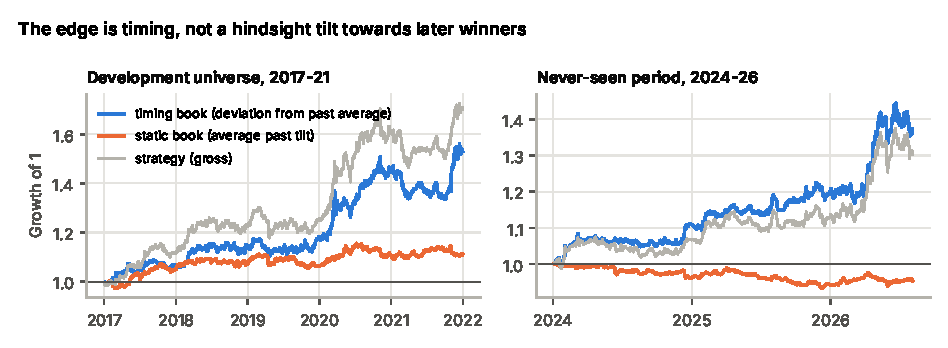
\includegraphics[width=\figw]{fig/fig13.pdf}
\caption{Causal decomposition of the gross book into a static book (each stock's expanding average of past weights) and a timing book (today's deviation from it). Both are tradable and add up to the strategy.}\label{fig:identity}
\end{figure}

\subsection{Implementation: delay, borrow, costs, smoothing and crash beta}

Four practical objections decide whether a paper alpha becomes a live loss. Table~\ref{tab:objections} and Figure~\ref{fig:implementation} report the full grid.
\begin{itemize}
  \item \emph{Execution delay:} Trading one session after the signal close leaves the development Sharpe ratio at 1.13, because each day only one forty-second of the book is re-targeted, a day's delay does not front-run information that builds over weeks
  \item \emph{Borrow and costs:} With a one-session delay, 10\,bp per unit traded and a 100\,bp annual borrow fee on all short notional, the Sharpe ratio is 1.06 (0.99 over the never-seen period). In the harshest cell of the grid (two sessions, 200\,bp borrow, 20\,bp costs) it is 0.96 and 0.89. The breakeven cost per unit traded is 234\,bp (197\,bp), the cleanest capacity diagnostic available without volume data and an order of magnitude above the cost of trading liquid large caps
  \item \emph{Smoothing:} Overlapping tranches smooth positions and not returns. The first-order autocorrelation of daily P\&L is 0.04 and the \citet{lo2002} autocorrelation-adjusted Sharpe ratio is 1.06 (1.06)
  \item \emph{Crash beta:} Weekly regressions with separate up- and down-market slopes give a down-market beta of $-0.07$ ($t = -1.24$) and an up-market beta of 0.03. In the worst decile of market weeks the book's average return is positive
\end{itemize}

\begin{figure}[t]
\centering
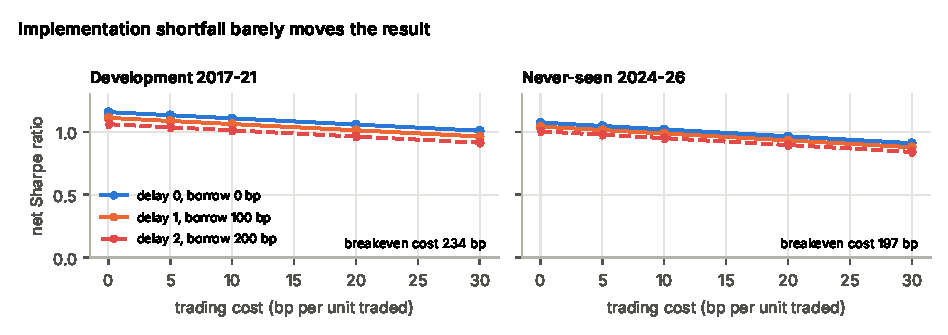
\includegraphics[width=\figw]{fig/fig14.pdf}
\caption{Net Sharpe ratio against trading cost in three implementation regimes: at the signal close without borrow fees, one session late with a 100\,bp borrow fee, two sessions late with a 200\,bp borrow fee.}\label{fig:implementation}
\end{figure}

\subsection{Research degrees of freedom}

A backtest has many choices (windows, thresholds, legs, tranches, allocators, signal sets, data rules), a result valid for one combination only is a search artefact. In the spirit of the multiverse analysis of \citet{steegen2016} and the specification curve of \citet{simonsohn2020}, I run the whole pipeline again over every choice in this research space. The grid covers the leader gap (5-20), the herd window (2-10 to 5-20), the LMH window (63-252), the breadth window, tranche length, legs, allocator, four signal sets, the information-event threshold (4-6), a two-session knowledge lag and the target expiry. The expiry choices include the quarterly 63-session horizon of the earnings cycle, as well as 126 and 252 sessions. Each parameter is moved one at a time, and 300 joint specifications are drawn at random.

Figure~\ref{fig:multiverse} shows three results.
\begin{itemize}
  \item \emph{The sign is not a choice:} 99\% of the development specifications and 97\% of the never-seen ones have a positive net Sharpe ratio (medians 0.80 and 0.72). The frozen specification is at the 98th percentile in development, as selection would imply, and at the 83rd out of sample, which selection would not
  \item \emph{The level depends on the choice:} Rankings inside the family do not persist (PBO 0.76). The ensemble of all specifications (no selection) has a Sharpe ratio of 0.92 over 2017-2021 ($t = 1.97$) and 0.86 out of sample, about 0.8 times the frozen specification
  \item \emph{Quarterly calibration and knowledge lag:} A hard 63-session expiry lowers the development Sharpe ratio to 0.94 (0.88 out of sample): dropping a target after one quarter throws away the information from analysts who update twice a year. Expiry at 126 sessions is equivalent to the 252-session default (1.12, 1.15). A two-session knowledge lag changes nothing (1.13, 1.06). Staleness is better handled inside the signal, by the event and silence clocks of LMH, than by cutting the snapshot short
\end{itemize}
Hansen's \citeyearpar{hansen2005} SPA test on a single window does not reject the null that no specification beats zero (development $p = 0.34$, never-seen $p = 0.14$, 2017-2021 ensemble $p = 0.095$). Section~\ref{sec:bayes} therefore combines the independent samples.

\begin{figure}[t]
\centering
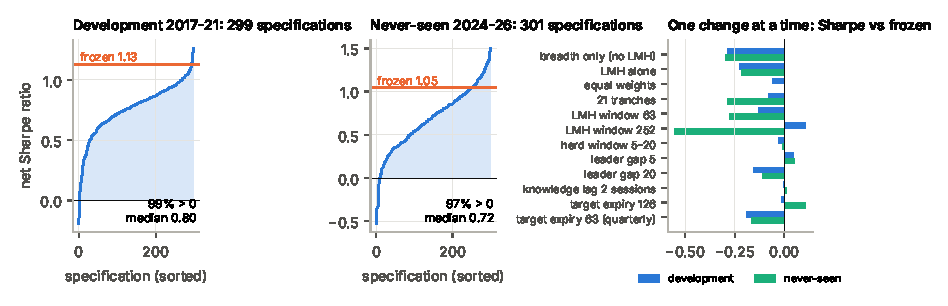
\includegraphics[width=\figw]{fig/fig15.pdf}
\caption{Left and centre: specification curves, i.e.\ the net Sharpe ratio of every randomly drawn specification sorted from worst to best, with the frozen specification marked. Right: change in Sharpe ratio when one choice at a time moves away from the frozen specification.}\label{fig:multiverse}
\end{figure}

\subsection{Multiple testing against the toolkit, and the marginal value of LMH}

Ranking first of 14 cross-sectional books (Section~\ref{sec:toolkit}) invites a charge of cherry-picking the comparison set. Two family-wise tests deal with it. The reverse SPA test asks whether any of the 16 institutional books significantly beats FMF-N once all are scaled to the same volatility, none does ($p = 0.86$ in sample, 0.86 out of sample). The \citet{romano2005} step-down procedure asks which books FMF-N beats under family-wise error control. In sample it beats 2 of 16, among them target-price momentum and 6-1 momentum. Out of sample no difference survives the correction, though 2 are individually significant. The defensible claim is ``never beaten, and better than most'', not ``significantly better than everything''.

The harder question is whether the new signal earns its place. Classic revision breadth is FMF's closest relative (correlation of the books 0.95). I compare FMF-N with the identical book built from the three breadth signals only, using a circular block bootstrap of paired returns \citep{ledoit2008}, the high correlation of the two books is what gives the test power. LMH adds 0.28 to the Sharpe ratio in development (95\% interval 0.03 to 0.54, $p = 0.028$) and 0.30 over the never-seen period ($-0.21$ to 0.80). Pooled, the gain is 0.29, with a posterior probability of 0.94 that it is positive.

\subsection{Small samples, done properly}\label{sec:bayes}

A $p$-value measures how surprising the data are under an effect of exactly zero. It ignores two facts an allocator would use. Most strategies fail, and here the same mechanism shows up in three independent samples, each with its own analysts and its own market path. Four Bayesian and small-sample tools are used (Figure~\ref{fig:bayes}).

\para{Posterior Sharpe ratios under sceptical priors:} The Bayesian bootstrap \citep{rubin1981} of weekly returns is a nonparametric posterior in which skewness and fat tails enter through the data, it is re-weighted by a prior on the annual Sharpe ratio. Under a sceptical $N(0,1)$ prior (most strategies have $|SR|<2$) the 2017-2021 posterior mean is 1.00 with $P(SR>0)=0.99$. Over the never-seen period it is 0.76 with $P(SR>0)=0.93$. Under a very sceptical $N(0,0.5)$ prior, which encodes the post-publication decay of anomalies documented by \citet{mclean2016}, the probabilities are 0.97 and 0.86.

\para{Random-effects meta-analysis across independent samples:} Development, holdout and the never-seen period are three non-overlapping samples of the same mechanism (the third adds twenty new names to the ten development names). A normal-normal random-effects model with a half-Cauchy prior on the between-sample heterogeneity $\tau$ \citep{gelman2006} pools them without assuming one common true effect. The LMH information coefficients are 0.095, 0.129 and 0.096. The pooled mean is 0.105 (90\% HDI 0.033 to 0.179), and the posterior-predictive probability of a positive IC in the next universe is 0.96. Stouffer's combination of the three one-sided $p$-values gives $p = 0.0022$, and the product of the three Bayes factors (prior sd 0.1) is 22. For the strategy's Sharpe ratio the pooled mean is 1.10 (90\% HDI 0.36 to 1.84), with $P(SR>0$ in the next universe$)=0.96$ and $P(SR>0.5)=0.86$.

\para{Shrinking the search:} In development LMH was the best of 18 candidate signals (Fama-MacBeth $t = 2.46$). Empirical-Bayes (James-Stein) shrinkage of the 18 $t$-statistics towards their family \citep{efron2010} brings this down to 1.06, with a posterior probability of 0.95 of a positive effect. This is what the development search is worth on its own: suggestive, not conclusive. It becomes evidence because the holdout and the never-seen period, which had no role in the search, gave the same information coefficient.

\para{Power:} With $N$ stocks and $M$ independent monthly cross-sections, the smallest mean IC detectable at 80\% power is $(z_{0.95}+z_{0.80})/\sqrt{(N-1)M}$ (Figure~\ref{fig:power}): 0.138 for ten stocks over three years, 0.077 for thirty, and 0.032 for a hundred stocks over five years. One ten-stock sample has a coin-flip chance (0.56) of detecting an IC of 0.10, so a null result in such a sample would tell us little. The never-seen period raises power to 0.91 and the three pooled samples go above 0.99. Monte Carlo on the calibrated generator agrees: with a true effect of the size in the data, the full pipeline finds it in 0.45 of ten-stock five-year worlds and 0.70 of thirty-stock worlds.

\begin{figure}[t]
\centering
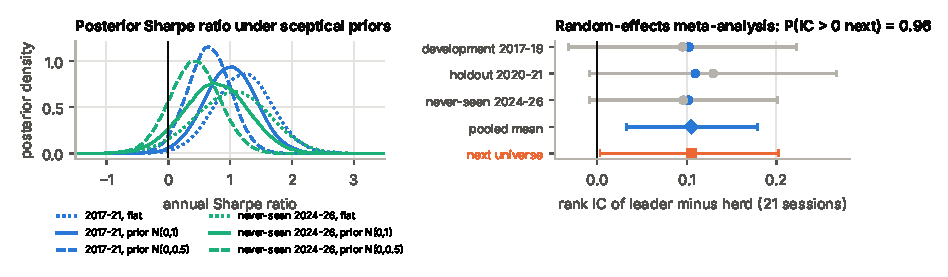
\includegraphics[width=\figw]{fig/fig16.pdf}
\caption{Left: posterior distributions of the annual Sharpe ratio (Bayesian bootstrap of weekly returns) under a flat prior and two sceptical priors. Right: random-effects meta-analysis of the leader-minus-herd IC. Grey: sample estimates with 95\% intervals, blue dots: partially pooled estimates, diamond: pooled mean (90\% HDI), square: predictive IC in a new universe.}\label{fig:bayes}
\end{figure}

\begin{figure}[t]
\centering
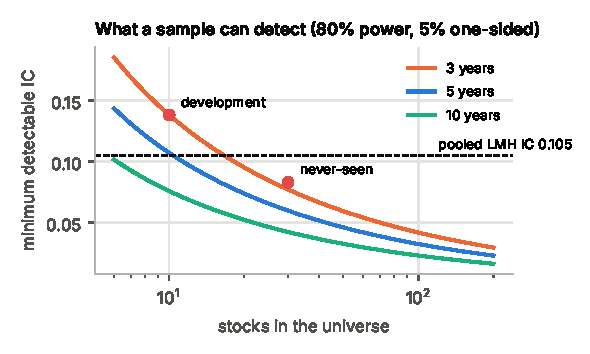
\includegraphics[width=0.62\textwidth]{fig/fig17.pdf}
\caption{Minimum detectable mean IC (80\% power, one-sided 5\%) by universe size and sample length. Red dots: the two universes of this paper. Dashed: the pooled LMH IC.}\label{fig:power}
\end{figure}

\section{Path risk: generative stress testing}\label{sec:generative}

A five-year history has one or two drawdown episodes, so the maximum drawdown and the Calmar ratio are close to single draws. To estimate their distribution I simulate many histories that keep what matters for drawdowns, namely fat tails, volatility clustering, and the nonlinear co-movement of the strategy with the market and with momentum.

\para{Four generators:} The generators are trained on the joint daily returns of FMF-N, the equal-weight market and the 12--1 momentum book, pooling the development period and the never-seen period after standardising each by its own mean and volatility ($\approx$1,900 days).
\begin{itemize}
  \item The stationary block bootstrap \citep{politis1994} re-orders history
  \item Filtered historical simulation \citep{baroneadesi1999} re-uses historical joint shock vectors inside GJR-GARCH-t volatility dynamics
  \item TimeGAN \citep{yoon2019} learns the whole path distribution adversarially
  \item Diffusion-FHS, the fourth, is a hybrid built for small samples. GJR-GARCH-t with variance targeting carries the volatility dynamics, for which five years of data are enough. A conditional denoising diffusion model \citep{ho2020} with a residual-MLP denoiser learns the joint law of the daily shock vector given the volatility regime, this is where flexibility pays off, and 1,900 observations of a three-dimensional vector are enough for it. The model can therefore draw shock combinations that history contains only rarely (for example a strategy loss together with a momentum crash in a high-volatility state) instead of replaying the few that happened. Gaussian-noise diffusion under-represents heavy tails when data are scarce, so the shocks are mapped to normal scores before training, with the Gaussian quantile transform of tabular diffusion \citep{kotelnikov2023}, and mapped back through the empirical quantile function with Student-t tails outside the sample. The diffusion model thus learns the regime-dependent dependence (a conditional copula), and the marginal tails come from the data
\end{itemize}
Early stopping on a chronologically held-out period selects the denoiser (without it, the network memorises the 1,900 training days and the draws collapse onto them). Sampling uses a strided DDIM-type chain \citep{song2021}. Daily moment matching \citep{boyle1997} removes small first- and second-moment biases of the sampler that would add up to a five-year drift. The GARCH parts use variance targeting \citep{engle1996}, with persistence capped at 0.99.

\para{Fidelity:} Table~\ref{tab:generative} gives the battery, with a discriminative score (gradient-boosting classifier on real vs synthetic 64-day windows, real windows split in time order to avoid leakage of overlapping windows) and a memorisation ratio. The block bootstrap matches the marginal moments by construction (strategy excess kurtosis 5.3 against 5.5) but can only re-order the days that happened. Diffusion-FHS has the lowest discriminative score of the generators (0.014, so the classifier can hardly tell its windows from real ones), a memorisation ratio of 0.96 (no copying) and a correlation with momentum of 0.62 against 0.66. Its tails are heavier than in the sample (strategy excess kurtosis 10.2 against 5.5, market 34 against 13): the GARCH recursion compounds rare large shocks into high-volatility spells longer than the five years happened to contain. For a stress test this is the cautious side to err on, and FHS goes much further (market excess kurtosis 63). TimeGAN fails. Its draws look Gaussian and are nearly collinear across channels (correlation with momentum 0.99), and a classifier separates them perfectly (score 0.500). This failure of adversarial training on short, noisy series is reported, not tuned away, and TimeGAN is left out of the inference.

\begin{table}[t]
\centering\footnotesize
\caption{Generative models: fidelity and path risk (pooled standardised samples, 1,000 five-year paths each)}\label{tab:generative}
\begin{adjustbox}{max width=\textwidth}\begin{tabular}{lrrrrrrr}
\toprule
 & FMF kurt. & MKT kurt. & corr(FMF, MOM) & Discrim. & Memoris. & Median Calmar & 5\% MaxDD (\%)\\
\midrule
Real data & 5.5 & 13 & 0.66 & -- & -- & -- & --\\
Block bootstrap & 5.3 & 13 & 0.67 & 0.067 & 0.97 & 0.91 & $-26$\\
FHS (GJR-GARCH-t) & 9.8 & 63 & 0.56 & 0.019 & 1.02 & 0.84 & $-29$\\
Diffusion-FHS & 10.2 & 34 & 0.62 & 0.014 & 0.96 & 0.70 & $-34$\\
TimeGAN & $-0.5$ & $-1$ & 0.99 & 0.500 & 1.11 & 1.26 & $-20$\\
\bottomrule
\end{tabular}\end{adjustbox}
\par\smallskip\begin{minipage}{0.97\textwidth}\footnotesize Discriminative score: $|\text{accuracy}-0.5|$ of a classifier separating real from synthetic windows (0 = indistinguishable). Memorisation ratio: nearest-training-window distance of synthetic windows relative to held-out real windows (1 = no copying). Calmar and drawdown use the posterior-predictive Sharpe ratio as drift.\end{minipage}
\end{table}

\para{Drift is an input:} No generator can learn a mean from five years of data. Paths have zero drift, and the strategy's drift is drawn from the posterior-predictive distribution of its Sharpe ratio in a new universe (Section~\ref{sec:bayes}), so parameter uncertainty and path risk enter the Calmar distribution together. Under Diffusion-FHS the median five-year Calmar ratio is 0.70, the probability of a Calmar ratio above 0.5 is 59\%, and the median maximum drawdown is $-15\%$ with a 5\% quantile of $-34\%$ (Figure~\ref{fig:generative}). The probability of losing money over five years is 14\%. An allocator should see these numbers rather than the single in-sample Calmar ratio.

\para{Conditional stress:} I look at simulated three-month windows. When the equal-weight market falls 25\% or more, FMF-N's mean return is positive under all generators: 6.4\% (bootstrap), 0.6\% (FHS), 10.9\% (Diffusion-FHS). When momentum has its worst 2\% of windows, the 5\% quantile of FMF-N's three-month return is between $-14.6\%$ and $-16.8\%$ (bootstrap $-14.1\%$), about twice the unconditional $-8.3\%$. So the risk to watch is momentum and not the market. The three generators get this tail in different ways (the bootstrap replays the 2020--21 momentum reversals, FHS rescales them with volatility dynamics, Diffusion-FHS draws new momentum-correlated shocks in high-volatility states) and still agree, which points to a property of the strategy. A PM can hedge momentum or cap momentum exposure when volatility is high, a QIS structurer should disclose the scenario.

\begin{figure}[t]
\centering
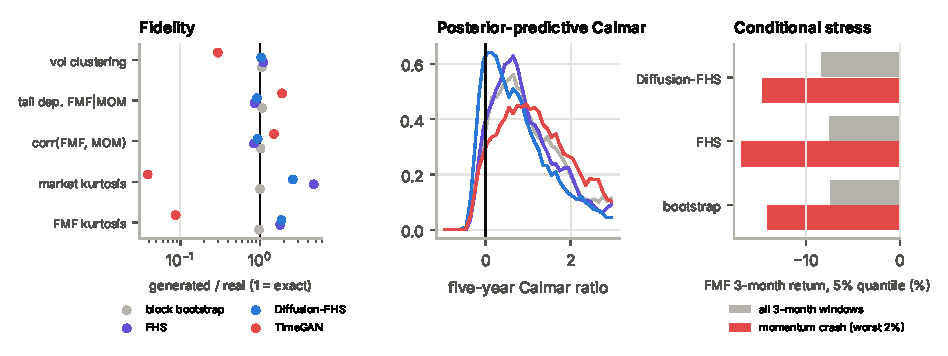
\includegraphics[width=\figw]{fig/fig18.pdf}
\caption{Left: stylised facts of real and generated data. Centre: distribution of the five-year Calmar ratio with posterior-predictive drift. Right: 5\% quantile of FMF-N's three-month return, unconditionally and in simulated momentum crashes.}\label{fig:generative}
\end{figure}

\section{Discussion: implications for practitioners}\label{sec:discussion}

\para{What holds up:} Four facts come back in the development sample, the holdout and a later, broader universe:
\begin{itemize}
  \item a zero-beta book built on revision flow has a Sharpe ratio near one after costs
  \item its alpha survives the market and the price factors
  \item leader minus herd predicts returns with an IC near 0.10
  \item the book improves almost any institutional strategy it is blended with, because its correlation with them is moderate and it behaves defensively in crises
\end{itemize}

\para{What does not hold up:} The construction cell is not identified (PBO 0.945, 0.76 over the multiverse). Deflated over the full research history the development Sharpe ratio is not significant, and neither is a family-wise test over all specifications on one short window. The circular time-shift placebo is passed only in the holdout, Section~\ref{sec:identity} relates this to the low power of that placebo, not to a hindsight tilt, and the placebo result is left as reported. In development, P\&L comes from a few names and days. Momentum crashes are the main stress. With ten stocks and a revision-based signal, these weaknesses are expected, the protocol is there to measure them.

\para{For portfolio managers:} FMF is a zero-beta selection sleeve, defensive in market crashes and exposed to momentum crashes. Three implementation choices follow.
\begin{itemize}
  \item \emph{Size on path risk:} The posterior-predictive drawdown distribution (5\% quantile $-34\%$ over five years) is a more realistic budget than the in-sample drawdown
  \item \emph{Decide beta explicitly:} Beta-neutral legs or a disclosed beta budget are one-line options in the package
  \item \emph{Monitor signal health:} The realised rolling IC is known in real time and gives early warning of decay
\end{itemize}
A breakeven cost of 234\,bp per unit traded and turnover of two to three times a year leave plenty of room for execution in liquid large caps.

\para{For QIS structurers:} The strategy is rules-based, uses only end-of-day data, and re-targets one forty-second of the book each day
\begin{itemize}
  \item \emph{Index delivery:} It can be delivered as an excess-return index with a volatility target, the package computes index levels, fees and a rulebook from the exact parameters
  \item \emph{Blending:} As a sleeve in a 50/50 combination it raises the Calmar ratio of every price-factor index studied, in and out of sample
  \item \emph{Disclosure:} The momentum-crash scenario of Section~\ref{sec:generative} is the stress scenario to disclose
\end{itemize}

\para{For researchers:} Three lessons apply beyond this strategy.
\begin{itemize}
  \item In small universes, report what a sample could detect before what it did detect
  \item Replace the single backtest with the family of reasonable backtests and a selection-free ensemble
  \item Combine independent samples formally, with a random-effects meta-analysis and its predictive distribution, instead of counting $p$-values below 0.05
\end{itemize}

\para{Implementation.:}
\begin{itemize}
  \item \emph{Inputs and execution:} Fully rules-based: end-of-day prices and target prices with a one-session knowledge lag, and one forty-second of the book re-targeted each session, which spreads execution
  \item \emph{Exposure and turnover:} Gross exposure about 0.9, net exposure zero, turnover two to three times a year
  \item \emph{Capacity:} Set by the liquidity of the names held. No volume data are used, but a breakeven cost of 234\,bp per unit traded leaves a wide margin for market impact in large caps
  \item \emph{Beta and blending:} Market exposure is a separate decision. With a constant beta budget of 0.2 the Calmar ratio over 2017--2021 rises to 1.66, above RTB's 1.39, with smaller drawdowns and no timing claim. For a QIS structurer the book is a natural low-correlation sleeve, and a 50/50 combination improves the drawdown profile of every price-factor index studied
\end{itemize}

\para{Limits:} Both universes are small, both cover mostly rising markets, and the out-of-sample window is 2.6 years. The out-of-sample universe (public Kaggle data, Section~\ref{sec:data}) is the ten development names plus twenty current large caps, the period is new, but the list of names was made with knowledge of which companies grew. The causal timing decomposition and the twenty-new-names check address this. An index-membership rule at the start of the window would be a better universe definition. Size, value and sector exposures need data not used here (the package has a sector-neutral option for users with a sector map). Next steps: a broad universe with analyst coverage, where the detectable IC is about 0.032, and a frozen live forward test.

\section{Conclusion}\label{sec:conclusion}

In a concentrated portfolio breadth is low and market exposure can inflate the reported Calmar ratio. I therefore separated the two. The selection signal adds to price momentum, the construction is matched to its information horizon, beta is a disclosed budget, and the tests are sized to the power of the sample. First-Mover Flow uses the timing of analyst revisions to build a zero-beta book. It does better than RTB and than the institutional comparables, improves blends with them, and replicates on a period and on twenty names not used in development. On the nine objections, it comes from timing and not from hindsight, it survives realistic implementation, and its sign does not depend on the specification. Pooled over independent samples, the probability that the mechanism works in the next universe is about 0.96.
The weak points are momentum crashes and the low precision of any single short sample. The list of failed hypotheses (Table~\ref{tab:ledger}) and the code, which reruns every test on another universe, are published with the paper.


\begin{thebibliography}{99}
\small
\setlength{\itemsep}{1pt}

\bibitem[Asquith, Mikhail, and Au(2005)]{asquith2005} Asquith, P., M.~B. Mikhail, and A.~S. Au, 2005, Information content of equity analyst reports, \emph{Journal of Financial Economics} 75, 245--282.
\bibitem[Bailey et~al.(2017)]{bailey2017} Bailey, D.~H., J.~M. Borwein, M. L\'opez de Prado, and Q.~J. Zhu, 2017, The probability of backtest overfitting, \emph{Journal of Computational Finance} 20, 39--69.
\bibitem[Bailey and L\'opez de Prado(2012)]{bailey2012} Bailey, D.~H., and M. L\'opez de Prado, 2012, The Sharpe ratio efficient frontier, \emph{Journal of Risk} 15, 3--44.
\bibitem[Bailey and L\'opez de Prado(2014)]{bailey2014} Bailey, D.~H., and M. L\'opez de Prado, 2014, The deflated Sharpe ratio: Correcting for selection bias, backtest overfitting, and non-normality, \emph{Journal of Portfolio Management} 40, 94--107.
\bibitem[Barone-Adesi, Giannopoulos, and Vosper(1999)]{baroneadesi1999} Barone-Adesi, G., K. Giannopoulos, and L. Vosper, 1999, VaR without correlations for portfolios of derivative securities, \emph{Journal of Futures Markets} 19, 583--602.
\bibitem[Barroso and Santa-Clara(2015)]{barroso2015} Barroso, P., and P. Santa-Clara, 2015, Momentum has its moments, \emph{Journal of Financial Economics} 116, 111--120.
\bibitem[Blitz, Huij, and Martens(2011)]{blitz2011} Blitz, D., J. Huij, and M. Martens, 2011, Residual momentum, \emph{Journal of Empirical Finance} 18, 506--521.
\bibitem[Boyle, Broadie, and Glasserman(1997)]{boyle1997} Boyle, P., M. Broadie, and P. Glasserman, 1997, Monte Carlo methods for security pricing, \emph{Journal of Economic Dynamics and Control} 21, 1267--1321.
\bibitem[Bradshaw, Brown, and Huang(2013)]{bradshaw2013} Bradshaw, M.~T., L.~D. Brown, and K. Huang, 2013, Do sell-side analysts exhibit differential target price forecasting ability?, \emph{Review of Accounting Studies} 18, 930--955.
\bibitem[Brav and Lehavy(2003)]{brav2003} Brav, A., and R. Lehavy, 2003, An empirical analysis of analysts' target prices: Short-term informativeness and long-term dynamics, \emph{Journal of Finance} 58, 1933--1967.
\bibitem[Chan, Jegadeesh, and Lakonishok(1996)]{chan1996} Chan, L.~K.~C., N. Jegadeesh, and J. Lakonishok, 1996, Momentum strategies, \emph{Journal of Finance} 51, 1681--1713.
\bibitem[Clarke, de~Silva, and Thorley(2002)]{clarke2002} Clarke, R., H. de~Silva, and S. Thorley, 2002, Portfolio constraints and the fundamental law of active management, \emph{Financial Analysts Journal} 58, 48--66.
\bibitem[Clement and Tse(2005)]{clement2005} Clement, M.~B., and S.~Y. Tse, 2005, Financial analyst characteristics and herding behavior in forecasting, \emph{Journal of Finance} 60, 307--341.
\bibitem[Cooper, Day, and Lewis(2001)]{cooper2001} Cooper, R.~A., T.~E. Day, and C.~M. Lewis, 2001, Following the leader: A study of individual analysts' earnings forecasts, \emph{Journal of Financial Economics} 61, 383--416.
\bibitem[Da and Schaumburg(2011)]{da2011} Da, Z., and E. Schaumburg, 2011, Relative valuation and analyst target price forecasts, \emph{Journal of Financial Markets} 14, 161--192.
\bibitem[DeMiguel, Garlappi, and Uppal(2009)]{demiguel2009} DeMiguel, V., L. Garlappi, and R. Uppal, 2009, Optimal versus naive diversification: How inefficient is the 1/N portfolio strategy?, \emph{Review of Financial Studies} 22, 1915--1953.
\bibitem[Diether, Malloy, and Scherbina(2002)]{diether2002} Diether, K.~B., C.~J. Malloy, and A. Scherbina, 2002, Differences of opinion and the cross section of stock returns, \emph{Journal of Finance} 57, 2113--2141.
\bibitem[Efron(2010)]{efron2010} Efron, B., 2010, \emph{Large-Scale Inference: Empirical Bayes Methods for Estimation, Testing, and Prediction} (Cambridge University Press, Cambridge).
\bibitem[Engle and Mezrich(1996)]{engle1996} Engle, R.~F., and J. Mezrich, 1996, GARCH for groups, \emph{Risk} 9, 36--40.
\bibitem[Fama and MacBeth(1973)]{fama1973} Fama, E.~F., and J.~D. MacBeth, 1973, Risk, return, and equilibrium: Empirical tests, \emph{Journal of Political Economy} 81, 607--636.
\bibitem[Frazzini and Pedersen(2014)]{frazzini2014} Frazzini, A., and L.~H. Pedersen, 2014, Betting against beta, \emph{Journal of Financial Economics} 111, 1--25.
\bibitem[Gelman(2006)]{gelman2006} Gelman, A., 2006, Prior distributions for variance parameters in hierarchical models, \emph{Bayesian Analysis} 1, 515--534.
\bibitem[George and Hwang(2004)]{george2004} George, T.~J., and C.-Y. Hwang, 2004, The 52-week high and momentum investing, \emph{Journal of Finance} 59, 2145--2176.
\bibitem[Gleason and Lee(2003)]{gleason2003} Gleason, C.~A., and C.~M.~C. Lee, 2003, Analyst forecast revisions and market price discovery, \emph{The Accounting Review} 78, 193--225.
\bibitem[Glosten, Jagannathan, and Runkle(1993)]{glosten1993} Glosten, L.~R., R. Jagannathan, and D.~E. Runkle, 1993, On the relation between the expected value and the volatility of the nominal excess return on stocks, \emph{Journal of Finance} 48, 1779--1801.
\bibitem[Grinold(1989)]{grinold1989} Grinold, R.~C., 1989, The fundamental law of active management, \emph{Journal of Portfolio Management} 15, 30--37.
\bibitem[Hamilton(1989)]{hamilton1989} Hamilton, J.~D., 1989, A new approach to the economic analysis of nonstationary time series and the business cycle, \emph{Econometrica} 57, 357--384.
\bibitem[Hansen(2005)]{hansen2005} Hansen, P.~R., 2005, A test for superior predictive ability, \emph{Journal of Business and Economic Statistics} 23, 365--380.
\bibitem[Harvey, Liu, and Zhu(2016)]{harvey2016} Harvey, C.~R., Y. Liu, and H. Zhu, 2016, \ldots and the cross-section of expected returns, \emph{Review of Financial Studies} 29, 5--68.
\bibitem[Henriksson and Merton(1981)]{henriksson1981} Henriksson, R.~D., and R.~C. Merton, 1981, On market timing and investment performance. II. Statistical procedures for evaluating forecasting skills, \emph{Journal of Business} 54, 513--533.
\bibitem[Ho, Jain, and Abbeel(2020)]{ho2020} Ho, J., A. Jain, and P. Abbeel, 2020, Denoising diffusion probabilistic models, \emph{Advances in Neural Information Processing Systems} 33, 6840--6851.
\bibitem[Holm(1979)]{holm1979} Holm, S., 1979, A simple sequentially rejective multiple test procedure, \emph{Scandinavian Journal of Statistics} 6, 65--70.
\bibitem[Hong, Kubik, and Solomon(2000)]{hong2000} Hong, H., J.~D. Kubik, and A. Solomon, 2000, Security analysts' career concerns and herding of earnings forecasts, \emph{RAND Journal of Economics} 31, 121--144.
\bibitem[Jegadeesh et~al.(2004)]{jegadeesh2004} Jegadeesh, N., J. Kim, S.~D. Krische, and C.~M.~C. Lee, 2004, Analyzing the analysts: When do recommendations add value?, \emph{Journal of Finance} 59, 1083--1124.
\bibitem[Jegadeesh and Titman(1993)]{jegadeesh1993} Jegadeesh, N., and S. Titman, 1993, Returns to buying winners and selling losers: Implications for stock market efficiency, \emph{Journal of Finance} 48, 65--91.
\bibitem[Jobson and Korkie(1981)]{jobson1981} Jobson, J.~D., and B.~M. Korkie, 1981, Performance hypothesis testing with the Sharpe and Treynor measures, \emph{Journal of Finance} 36, 889--908.
\bibitem[Kotelnikov et~al.(2023)]{kotelnikov2023} Kotelnikov, A., D. Baranchuk, I. Rubachev, and A. Babenko, 2023, TabDDPM: Modelling tabular data with diffusion models, \emph{Proceedings of the 40th International Conference on Machine Learning}, 17564--17579.
\bibitem[Ledoit and Wolf(2008)]{ledoit2008} Ledoit, O., and M. Wolf, 2008, Robust performance hypothesis testing with the Sharpe ratio, \emph{Journal of Empirical Finance} 15, 850--859.
\bibitem[Lo(2002)]{lo2002} Lo, A.~W., 2002, The statistics of Sharpe ratios, \emph{Financial Analysts Journal} 58, 36--52.
\bibitem[Lo(2008)]{lo2008} Lo, A.~W., 2008, Where do alphas come from? A measure of the value of active investment management, \emph{Journal of Investment Management} 6, 1--29.
\bibitem[L\'opez de Prado(2018)]{lopezdeprado2018} L\'opez de Prado, M., 2018, \emph{Advances in Financial Machine Learning} (Wiley, Hoboken, NJ).
\bibitem[McLean and Pontiff(2016)]{mclean2016} McLean, R.~D., and J. Pontiff, 2016, Does academic research destroy stock return predictability?, \emph{Journal of Finance} 71, 5--32.
\bibitem[Memmel(2003)]{memmel2003} Memmel, C., 2003, Performance hypothesis testing with the Sharpe ratio, \emph{Finance Letters} 1, 21--23.
\bibitem[Moreira and Muir(2017)]{moreira2017} Moreira, A., and T. Muir, 2017, Volatility-managed portfolios, \emph{Journal of Finance} 72, 1611--1644.
\bibitem[Moskowitz, Ooi, and Pedersen(2012)]{moskowitz2012} Moskowitz, T.~J., Y.~H. Ooi, and L.~H. Pedersen, 2012, Time series momentum, \emph{Journal of Financial Economics} 104, 228--250.
\bibitem[Newey and West(1987)]{newey1987} Newey, W.~K., and K.~D. West, 1987, A simple, positive semi-definite, heteroskedasticity and autocorrelation consistent covariance matrix, \emph{Econometrica} 55, 703--708.
\bibitem[Nichol and Dhariwal(2021)]{nichol2021} Nichol, A.~Q., and P. Dhariwal, 2021, Improved denoising diffusion probabilistic models, \emph{Proceedings of the 38th International Conference on Machine Learning}, 8162--8171.
\bibitem[Novy-Marx and Velikov(2016)]{novymarx2016} Novy-Marx, R., and M. Velikov, 2016, A taxonomy of anomalies and their trading costs, \emph{Review of Financial Studies} 29, 104--147.
\bibitem[Politis and Romano(1994)]{politis1994} Politis, D.~N., and J.~P. Romano, 1994, The stationary bootstrap, \emph{Journal of the American Statistical Association} 89, 1303--1313.
\bibitem[Romano and Wolf(2005)]{romano2005} Romano, J.~P., and M. Wolf, 2005, Stepwise multiple testing as formalized data snooping, \emph{Econometrica} 73, 1237--1282.
\bibitem[Rubin(1981)]{rubin1981} Rubin, D.~B., 1981, The Bayesian bootstrap, \emph{Annals of Statistics} 9, 130--134.
\bibitem[Simonsohn, Simmons, and Nelson(2020)]{simonsohn2020} Simonsohn, U., J.~P. Simmons, and L.~D. Nelson, 2020, Specification curve analysis, \emph{Nature Human Behaviour} 4, 1208--1214.
\bibitem[Song, Meng, and Ermon(2021)]{song2021} Song, J., C. Meng, and S. Ermon, 2021, Denoising diffusion implicit models, \emph{International Conference on Learning Representations}.
\bibitem[Steegen et~al.(2016)]{steegen2016} Steegen, S., F. Tuerlinckx, A. Gelman, and W. Vanpaemel, 2016, Increasing transparency through a multiverse analysis, \emph{Perspectives on Psychological Science} 11, 702--712.
\bibitem[Stickel(1991)]{stickel1991} Stickel, S.~E., 1991, Common stock returns surrounding earnings forecast revisions: More puzzling evidence, \emph{The Accounting Review} 66, 402--416.
\bibitem[Treynor and Mazuy(1966)]{treynor1966} Treynor, J., and K. Mazuy, 1966, Can mutual funds outguess the market?, \emph{Harvard Business Review} 44, 131--136.
\bibitem[Welch(2000)]{welch2000} Welch, I., 2000, Herding among security analysts, \emph{Journal of Financial Economics} 58, 369--396.
\bibitem[White(2000)]{white2000} White, H., 2000, A reality check for data snooping, \emph{Econometrica} 68, 1097--1126.
\bibitem[Wiese et~al.(2020)]{wiese2020} Wiese, M., R. Knobloch, R. Korn, and P. Kretschmer, 2020, Quant GANs: Deep generation of financial time series, \emph{Quantitative Finance} 20, 1419--1440.
\bibitem[Yoon, Jarrett, and van~der Schaar(2019)]{yoon2019} Yoon, J., D. Jarrett, and M. van~der Schaar, 2019, Time-series generative adversarial networks, \emph{Advances in Neural Information Processing Systems} 32, 5508--5518.
\end{thebibliography}


\appendix
\section{Data cleaning log (development universe)}\label{app:cleaning}

\begin{table}[h]
\centering\small
\begin{adjustbox}{max width=\textwidth}\begin{tabular}{lllr}
\toprule
Dataset & Check & Action & Rows\\
\midrule
Prices & clean & Non-sessions removed (coverage $<50\%$) & 55\\
Ratings & R1 & Unparseable / non-positive target & 9\\
Ratings & R2 & Missing analyst identifier & 47\\
Ratings & R3 & TP/P outside (0.2, 5.0) & 2\\
Ratings & R4 & Target change inconsistent with price change (excess outside (0.33, 3.0)) & 0\\
\bottomrule
\end{tabular}\end{adjustbox}
\par\smallskip\begin{minipage}{0.9\textwidth}\footnotesize Over the never-seen period the same rules remove eight ratings published after the last session and two implausible targets.\end{minipage}
\end{table}

\section{Signal and comparable definitions}\label{app:defs}

Every signal is oriented so that higher is more attractive, and uses data known at $t$. Price signals: 12-1 momentum $\ln P_{t-21}-\ln P_{t-252}$, 6-1 momentum $\ln P_{t-21}-\ln P_{t-126}$, reversal $-(\ln P_t-\ln P_{t-21})$, low volatility $-\mathrm{sd}_{60}(r)$, betting-against-beta $-\hat\beta_{252}$ on the equal-weight market, residual momentum, the 231-session sum of market-residual returns divided by their standard deviation and lagged 21 sessions, 52-week high $P_t/\max_{252}P$. Analyst signals: consensus upside $\ln(\mathrm{median}\,TP/P)$, target-price momentum $\Delta_{63}\ln(\mathrm{median}\,TP)$, low dispersion $-\mathrm{sd}(\ln TP)$, classic breadth $B_{i,t}$. Blends: equal-weight ranks of (12-1 momentum, low volatility, reversal) and of (12-1 momentum, breadth). Allocations: equal-weight and inverse-60-day-volatility long-only, time-series momentum (long or short each stock by the sign of its 12-1 return, rebalanced monthly).

\section{Pre-registrations}\label{app:prereg}

The hypotheses of each audit round and the out-of-sample transfer rules were serialised to JSON and hashed (SHA-256, first 16 hexadecimal characters) before any outcome was computed. The notebook verifies the out-of-sample file (\texttt{configs/oos\_open\_universe\_preregistration.json}, hash \texttt{0b2b0792fd357d61}) before printing any result. The file fixes the frozen parameters, the primary and secondary leg rules, the warm-up, the evaluation window, the list of tests, and the rule that nothing is changed afterwards.

\section{Development universe identification}

From my reconciliation of return signatures against public closing prices, the ten development series are large US technology, consumer, industrial and financial names (stock\_1 AAPL, stock\_2 BA, stock\_3 CHGG, stock\_4 INTC, stock\_5 JPM, stock\_6 MSFT, stock\_7 NKE, stock\_8 NVDA, stock\_9 PANW, stock\_10 QCOM). The identification serves only for interpretation, no rule uses it.

\section{Generative models: specification}

\para{Diffusion-FHS:} For each channel $c$ (FMF-N, equal-weight market, 12--1 momentum book), standardised returns $x_{c,t}$ follow a GJR-GARCH(1,1) recursion $\sigma^2_{c,t+1}=\omega_c+(\alpha_c+\gamma_c\mathbf 1_{e_{c,t}<0})e^2_{c,t}+\beta_c\sigma^2_{c,t}$, with $e_{c,t}=\sigma_{c,t}z_{c,t}$. The parameters $(\alpha,\gamma,\beta)$ are estimated by Student-t quasi-likelihood on the pooled samples, persistence is capped at 0.99, and $\omega$ is set by variance targeting. A conditional DDPM learns $p(u_t\mid c_t)$, where $u_t\in\mathbb R^3$ are the normal scores of the innovation vector $z_t$ (rank-based Gaussian quantile transform) and $c_t$ is the vector of standardised log volatilities. Draws go back to $z_t$ through the empirical quantile functions, extended beyond the sample with standardised Student-t tails using the GARCH degrees of freedom. Denoiser: residual MLP, three blocks of width 128, SiLU, sinusoidal time embedding. Training: cosine schedule with $T=100$ steps \citep{nichol2021}, simplified $\epsilon$-prediction loss, Adam with warm-up and cosine decay, EMA of weights at 0.999, early stopping on the last 15\% of each sample. To simulate, I alternate one step of the GARCH recursion with a 50-step strided ancestral sampler \citep{song2021} that takes the current volatility state as its condition. Each day the shock vectors are moment-matched across paths (mean zero, empirical standard deviation). Volatility states may not leave the observed range plus half a standard deviation on each side.

\para{Baselines:} The stationary bootstrap has a mean block of 21 days. FHS uses the same GJR-GARCH dynamics with empirical residual vectors resampled jointly. TimeGAN follows \citet{yoon2019}, with single-layer GRUs (hidden size 24), 24-day windows, and 1,500 embedding, 1,500 supervised and 2,000 joint iterations.

\para{Fidelity battery:} Moments, the autocorrelation of absolute returns (lags 1--10), cross-correlations and 5\% tail dependence, a discriminative score from a gradient-boosting classifier on window features and raw values, with real windows split in time order and a one-window gap, and a memorisation ratio from Euclidean nearest-neighbour distances to training windows relative to held-out real windows.

\section{Software architecture}

The package \texttt{fmflow} is organised by responsibility:
\begin{itemize}
  \item \texttt{data}: the contract, cleaning with an audit log, and the point-in-time snapshot
  \item \texttt{signals}: the registry of built-in and user signals
  \item \texttt{risk}: walk-forward GJR-GARCH and an on-disk cache
  \item \texttt{portfolio}: legs, allocators, beta neutrality, caps, volatility targeting and tranches
  \item \texttt{backtest}: costs, borrow and execution delay
  \item \texttt{analytics}: metrics, inference, snooping-robust tests, Bayesian tools, attribution and power
  \item \texttt{robustness}: placebos, leave-one-out, the multiverse and truncation checks
  \item \texttt{generative}, \texttt{production} (book, trades, risk report, signal monitor) and \texttt{index} (QIS index levels and rulebook)
\end{itemize}
All tunable numbers sit in two frozen configuration classes that serialise to JSON and can be fingerprinted before evaluation. A command-line interface exposes the workflows. Ten notebooks cover data ingestion, signal research, construction and risk, robustness and inference, generative stress testing, QIS index construction, the PM's daily workflow and a full pre-registered research cycle on a user's own universe.

\section{Reproducibility}

The repository (\texttt{first-mover-flow}) contains a self-contained Python package, \texttt{fmflow}. It runs the full pipeline from two raw tables (daily prices, analyst target prices with publication dates) to daily weights and net returns, with modules for the data contract and audited cleaning, the point-in-time snapshot, signals, GJR-GARCH risk, portfolio construction and the backtest. The validation battery of this paper is included: phase-averaged IC tests, PSR/DSR, CSCV, placebos through the identical construction, leave-one-out rebuilds, the 13 institutional comparables and three allocations, and a pre-registration utility that fingerprints a specification before evaluation. A structural synthetic data generator, calibrated to both universes, checks that the pipeline finds no alpha in a null world. More than 100 unit, causality (truncation) and parity tests run in continuous integration on Linux and Windows. With the notebook's GARCH forecasts the package reproduces the research notebook's weights to within $5\times10^{-13}$ on the open universe, and exactly on the development universe on the machine that produced them. The development forecasts come from the proprietary prices and are not distributed, re-estimated on a second machine they move the weights by at most 0.019 and the 2017--2021 Sharpe ratio by less than 0.01, with the same names long and short every day. Re-estimating GARCH from scratch is exact on one machine but not across machines. On a few hundred observations the GJR-GARCH-t likelihood has local maxima of nearly equal height, and where a gradient optimiser stops depends on the floating-point path of the processor (a different BLAS kernel moves the out-of-sample Sharpe ratio from 1.05 to 1.02). The package therefore also has a deterministic grid-likelihood estimator with variance targeting, it is bit-identical across machines and gives Sharpe ratios of 1.09 out of sample and 1.12 over 2017--2021. The open data, the notebook that rebuilds them from public sources, and the registration file are distributed. The proprietary development data are not.

\end{document}
